%%% LaTeX-Vorlage Version 1.8 %%%

% Grundlegende Dokumenteneigenschaften gemäß DHBW-Vorgaben
\documentclass[a4paper,fontsize=11pt,oneside,parskip=half,headings=normal]{scrreprt} 
% \usepackage{showframe} % nur für Kontrolle der Ränder 

%%% Präambel einbinden (mit Festlegungen gemäß DHBW-Vorgaben) %%%
%%% Präambel %%%
% hier sollten keine Änderungen erforderlich sein
%
\usepackage[utf8]{inputenc}   % Zeichencodierung UTF-8 für Eingabe-Dateien
\usepackage[T1]{fontenc}      % Darstellung von Umlauten im PDF

\usepackage{listings}         % für Einbindung von Code-Listings
\lstset{numbers=left,numberstyle=\tiny,numbersep=5pt,texcl=true}
\lstset{literate=             % erlaubt Sonderzeichen in Code-Listings 
{Ö}{{\"O}}1
{Ä}{{\"A}}1
{Ü}{{\"U}}1
{ß}{{\ss}}2
{ü}{{\"u}}1
{ä}{{\"a}}1
{ö}{{\"o}}1
{€}{{\euro}}1
}

\usepackage[
  inner=35mm,outer=15mm,top=25mm,
  bottom=20mm,foot=12mm,includefoot
]{geometry}                 % Einstellungen für Ränder

\usepackage[english]{babel} % Spracheinstellungen Englisch
\usepackage[babel,english=british]{csquotes} % englische Anf.zeichen
\usepackage{enumerate}      % anpassbare Nummerier./Aufz.
\usepackage{graphicx}       % Einbinden von Grafiken
\usepackage[onehalfspacing]{setspace} % anderthalbzeilig

\usepackage{blindtext}      % Textgenerierung für Testzwecke
\usepackage{color}          % Verwendung von Farbe 

\usepackage{acronym}        % für ein Abkürzungsverzeichnis

\usepackage[                % Biblatex
  backend=biber,
  bibstyle=_dhbw_authoryear,maxbibnames=99,
  citestyle=authoryear,     
  uniquename=true, useprefix=true,
  bibencoding=utf8]{biblatex}
%kein Punkt am Ende bei \footcite
%http://www.golatex.de/footcite-ohne-punkt-am-schluss-t4865.html
\renewcommand{\bibfootnotewrapper}[1]{\bibsentence#1}


%Reihenfolge der Autorennamen
%   
% http://golatex.de/viewtopic,p,80448.html#80448
% Argumente: siehe http://texwelt.de/blog/modifizieren-eines-biblatex-stils/
\DeclareNameFormat{sortname}{% Bibliographie
  \ifnum\value{uniquename}=0 % Normalfall
    \ifuseprefix%
      {%
         \usebibmacro{name:family-given}
           {\namepartfamily}
           {\namepartgiveni}
           {\namepartprefix}
           {\namepartsuffixi}%
       }
      {%
         \usebibmacro{name:family-given}
           {\namepartfamily}
           {\namepartgiveni}
           {\namepartprefixi}
           {\namepartsuffixi}%
       }%
  \fi
  \ifnum\value{uniquename}=1% falls nicht eindeutig, abgek. Vorname 
      {%
         \usebibmacro{name:family-given}
           {\namepartfamily}
           {\namepartgiveni}
           {\namepartprefix}
           {\namepartsuffix}%
       }%
  \fi
  \ifnum\value{uniquename}=2% falls nicht eindeutig, ganzer Vorname 
      {%
         \usebibmacro{name:family-given}
           {\namepartfamily}
           {\namepartgiven}
           {\namepartprefix}
           {\namepartsuffix}%
       }%
  \fi   
  \usebibmacro{name:andothers}}

\DeclareNameFormat{labelname}{% für Zitate
  \ifnum\value{uniquename}=0 % Normalfall
    \ifuseprefix%
      {%
         \usebibmacro{name:family-given}
           {\namepartfamily}
           {\empty}
           {\namepartprefix}
           {\namepartsuffixi}%
       }
      {%
         \usebibmacro{name:family-given}
           {\namepartfamily}
           {\empty}
           {\namepartprefixi}
           {\namepartsuffixi}%
       }%
  \fi
  \ifnum\value{uniquename}=1% falls nicht eindeutig, abgek. Vorname 
      {%
         \usebibmacro{name:family-given}
           {\namepartfamily}
           {\namepartgiveni}
           {\namepartprefix}
           {\namepartsuffix}%
       }%
  \fi
  \ifnum\value{uniquename}=2% falls nicht eindeutig, ganzer Vorname 
      {%
         \usebibmacro{name:family-given}
           {\namepartfamily}
           {\namepartgiven}
           {\namepartprefix}
           {\namepartsuffix}%
       }%
  \fi   
  \usebibmacro{name:andothers}}
      
  
\DeclareFieldFormat{extrayear}{% = the 'a' in 'Jones 1995a'
  \iffieldnums{labelyear}
    {\mknumalph{#1}}
    {\mknumalph{#1}}}        

\renewcommand*{\multinamedelim}{\addslash}
\renewcommand*{\finalnamedelim}{\addslash}
\renewcommand*{\multilistdelim}{\addslash}
\renewcommand*{\finallistdelim}{\addslash}

\renewcommand{\nameyeardelim}{~}

% Literaturverzeichnis: Doppelpunkt zwischen Name (Jahr): Rest 
% http://de.comp.text.tex.narkive.com/Tn1HUIXB/biblatex-authoryear-und-doppelpunkt
\renewcommand{\labelnamepunct}{\addcolon\addspace}

% damit die Darstellung für Vollzitate von Primärquellen in 
% Fußnoten später auf "nicht fett" geändert werden kann 
% (nur für Zitate von Sekundärliteratur relevant)
\newcommand{\textfett}[1]{\textbf{#1}}

% für Zitate von Sekundärliteratur:
\newcommand{\footcitePrimaerSekundaer}[4]{%
  \renewcommand{\textfett}[1]{##1}%
  \footnote{\fullcite[#2]{#1}, zitiert nach \cite[#4]{#3}}%  
  \renewcommand{\textfett}[1]{\textbf{##1}}%
}

% Im Literaturverzeichnis: Autor (Jahr) fett
\renewbibmacro*{author}{%
  \ifboolexpr{%
    test \ifuseauthor%
    and
    not test {\ifnameundef{author}}
  }
    {\usebibmacro{bbx:dashcheck}
       {\bibnamedash}
       {\usebibmacro{bbx:savehash}%
        \textfett{\printnames{author}}%
        \iffieldundef{authortype}
          {\setunit{\addspace}}
          {\setunit{\addcomma\space}}}%
     \iffieldundef{authortype}
       {}
       {\usebibmacro{authorstrg}%
        \setunit{\addspace}}}%
    {\global\undef\bbx@lasthash
     \usebibmacro{labeltitle}%
     \setunit*{\addspace}}%
  \textfett{\usebibmacro{date+extrayear}}}

% Sonderfall: Quelle ohne Autor, aber mit Herausgeber
% Name des Herausgebers wird fett gedruckt
\renewbibmacro*{bbx:editor}[1]{%
  \ifboolexpr{%
    test \ifuseeditor%
    and
    not test {\ifnameundef{editor}}
  }
    {\usebibmacro{bbx:dashcheck}
       {\bibnamedash}
       {\textfett{\printnames{editor}}%
        \setunit{\addcomma\space}%
        \usebibmacro{bbx:savehash}}%
     \usebibmacro{#1}%
     \clearname{editor}%
     \setunit{\addspace}}%
    {\global\undef\bbx@lasthash
     \usebibmacro{labeltitle}%
     \setunit*{\addspace}}%
  \textfett{\usebibmacro{date+extrayear}}}

% Anpassungen für deutsche Sprache
\DefineBibliographyStrings{english}{%
	nodate = {{o.J.}},
	urlseen = {{Abruf:}},
	ibidem = {{ebenda}}
}

% keine Anführungszeichen beim Titel im Literaturverzeichnis
\DeclareFieldFormat[article,book,inbook,inproceedings,manual,misc,phdthesis,thesis,online,report]{title}{#1\isdot}

\newcommand{\literaturverzeichnis}{%
% nur Literaturverzeichnis
% (als eigenes Kapitel)
\phantomsection
\addcontentsline{toc}{chapter}{List of literature}
\spezialkopfzeile{List of literature}
\defbibheading{lit}{\section*{List of literature}}
\label{chapter:quellen}
\printbibliography[heading=lit,notkeyword=ausblenden]
}

% Anpassungen für englische Sprache
\DefineBibliographyStrings{english}{
    nodate = {{w.y.}},
    urlseen = {{retrieval:}}
} % mit DHBW-spezifischen Einstellungen

\usepackage{hyperref}       % URL-Formatierung, klickbare Verweise

\usepackage{tocloft}        % für Verzeichnis der Anhänge

\usepackage{graphicx}       % Einbinden von Grafiken
\usepackage{tikz}           %  -"-

\newcounter{anhcnt}
\setcounter{anhcnt}{0}
\newlistof{anhang}{app}{}

\newcommand{\anhang}[1]{%
  \refstepcounter{anhcnt}
  \setcounter{anhteilcnt}{0}
  \section*{Appendix \theanhcnt: #1}
  \addcontentsline{app}{section}{\protect\numberline{Anhang \theanhcnt}#1}\par
}

\newcounter{anhteilcnt}
\setcounter{anhteilcnt}{0}

\newcommand{\comment}[1]{} % Ermoeglicht das einfuegen von commentaren, die nicht gerendert werden

\newcommand{\anhangteil}[1]{%
	\refstepcounter{anhteilcnt}
	\subsection*{Anhang~\arabic{anhcnt}/\arabic{anhteilcnt}: #1}
	\addcontentsline{app}{subsection}{\protect\numberline{Anhang \theanhcnt/\arabic{anhteilcnt}}#1}\par
}

\renewcommand{\theanhteilcnt}{Anhang \theanhcnt/\arabic{anhteilcnt}}

% vgl. S. 4 Paket-Beschreibung tocloft 	
% Einrückungen für Anhangverzeichnis
\makeatletter
\newcommand{\abstaendeanhangverzeichnis}{
\renewcommand*{\l@section}{\@dottedtocline{1}{0em}{5.5em}}
\renewcommand*{\l@subsection}{\@dottedtocline{2}{2.3em}{6.5em}}
}
\makeatother

% Abbildungs- und Tabellenverzeichnis
% Bezeichnungen
\renewcaptionname{english}{\figurename}{Abb.}
\renewcaptionname{english}{\tablename}{Tab.}
% Einrückungen
\makeatletter
\renewcommand*{\l@figure}{\@dottedtocline{1}{0em}{2.3em}}
\renewcommand*{\l@table}{\@dottedtocline{1}{0em}{2.3em}}
\makeatother


\usepackage{chngcntr}                % fortlaufende Zähler für Fußnoten, Abbildungen und Tabellen
\counterwithout{figure}{chapter}
\counterwithout{table}{chapter}
\counterwithout{footnote}{chapter}

\usepackage[automark]{scrlayer-scrpage} 
%% Definitionen für Kopf- und Fußzeile auf normalen Seiten
\defpagestyle{kopfzeile}
{% Kopfdefinition
  (\textwidth,0pt)    % Länge der oberen Linie,Dicke der oberen Linie       
  {} % Definition für linke Seiten im doppelseitigen Layout
  {} % Definition für rechte Seiten im doppelseitigen Layout      
  {  % Definition für Seiten im einseitigen Layout
	\makebox[0pt][l]{\rightmark}% 
	\makebox[\linewidth]{}% 
  }        
  (\textwidth, 0.4pt) % Untere Linienlänge, Untere Liniendicke
}
{% Fußdefinition
  (\textwidth,0pt)    % Obere Linienlänge, Obere Liniendicke
  {} % Definition für linke Seiten im doppelseitigen Layout
  {} % Definition für rechte Seiten im doppelseitigen Layout
  {  % Definition für Seiten im einseitigen Layout
    \makebox[\linewidth]{}%
    \makebox[0pt][r]{\pagemark}%
  }
  (\textwidth, 0pt)   % Länge der unteren Linie,Dicke der unteren Linie
}

%% Definitionen für Kopf- und Fußzeile auf ersten Seiten eines Kapitels
\defpagestyle{kapitelkopfzeile}
{% Kopfdefinition
  (\textwidth,0pt)    % Länge der oberen Linie,Dicke der oberen Linie       
  {} % Definition für linke Seiten im doppelseitigen Layout
  {} % Definition für rechte Seiten im doppelseitigen Layout      
  {}  % Definition für Seiten im einseitigen Layout
  (\textwidth, 0pt) % Untere Linienlänge, Untere Liniendicke
}
{% Fußdefinition
  (\textwidth,0pt)    % Obere Linienlänge, Obere Liniendicke
  {} % Definition für linke Seiten im doppelseitigen Layout
  {} % Definition für rechte Seiten im doppelseitigen Layout
  {  % Definition für Seiten im einseitigen Layout
    \makebox[\linewidth]{}%
    \makebox[0pt][r]{\pagemark}%
  }
  (\textwidth, 0pt)   % Länge der unteren Linie,Dicke der unteren Linie
}

%% Definitionen für Kopf- und Fußzeile im Anhang und bei Quellenverzeichnisse
\newcommand{\spezialkopfzeileBezeichnung}{}
\defpagestyle{spezialkopfzeile}
{% Kopfdefinition
  (\textwidth,0pt)    % Länge der oberen Linie,Dicke der oberen Linie       
  {} % Definition für linke Seiten im doppelseitigen Layout
  {} % Definition für rechte Seiten im doppelseitigen Layout      
  {  % Definition für Seiten im einseitigen Layout
	\makebox[0pt][l]{\spezialkopfzeileBezeichnung}% 
	\makebox[\linewidth]{}% 
  }        
  (\textwidth, 0.4pt) % Untere Linienlänge, Untere Liniendicke
}
{% Fußdefinition
  (\textwidth,0pt)    % Obere Linienlänge, Obere Liniendicke
  {} % Definition für linke Seiten im doppelseitigen Layout
  {} % Definition für rechte Seiten im doppelseitigen Layout
  {  % Definition für Seiten im einseitigen Layout
    \makebox[\linewidth]{}%
    \makebox[0pt][r]{\pagemark}%
  }
  (\textwidth, 0pt)   % Länge der unteren Linie,Dicke der unteren Linie
}
            
\newcommand\spezialkopfzeile[1]{%
  \renewcommand\spezialkopfzeileBezeichnung{#1}
  \pagestyle{spezialkopfzeile}
}
                
% Standard-Pagestyle auswählen
\pagestyle{kopfzeile}

% keine Kopfzeile anzeigen auf Seiten, auf denen ein 
% Kapitel beginnt oder das Inhalts-/Abbildungs-/Tabellenverzeichnis steht 
\renewcommand{\chapterpagestyle}{kapitelkopfzeile}
\tocloftpagestyle{kapitelkopfzeile}

		 % für schöne Kopfzeilen 

\usepackage{textcomp}            % erlaubt EUR-Zeichen in Eingabedatei
\usepackage{eurosym}             % offizielles EUR-Symbol in Ausgabe
\renewcommand{\texteuro}{\euro}  % ACHTUNG: nach hyperref aufrufen!

\usepackage{scrhack}             % stellt Kompatibilität zw. KOMA-Script
                                 % (scrreprt) und anderen Paketen her
                                 
% Anpassung der Abstände bei Kapitelüberschriften
% (betrifft auch Inhalts-, Abbildungs- und Tabellenverzeichnis)
\renewcommand*\chapterheadstartvskip{\vspace*{-\topskip}}
\newcommand{\myBeforeTitleSkip}{1mm}
\newcommand{\myAfterTitleSkip}{10mm}
\setlength\cftbeforetoctitleskip{\myBeforeTitleSkip}
\setlength\cftbeforeloftitleskip{\myBeforeTitleSkip}
\setlength\cftbeforelottitleskip{\myBeforeTitleSkip}

\setlength\cftaftertoctitleskip{\myAfterTitleSkip}
\setlength\cftafterloftitleskip{\myAfterTitleSkip}
\setlength\cftafterlottitleskip{\myAfterTitleSkip}                                                            
%%% Ende der Präambel %%%

%%% Name der eigenen Literatur-Datenbank (ggf. anpassen) %%%
\bibliography{includes/boilerplate/literatur-datenbank.bib}
\bibliography{includes/boilerplate/literatur-datenbank_win.bib}

\begin{document}
%%% Deckblatt einbinden %%% 
% Anpassungen nötig (Name, Titel etc.)
% HIER EDITIEREN: 
% Typ der Arbeit (für Deckblatt und ehrenwörtliche Erklärung)
% - bitte Zutreffendes auswählen
\newcommand{\typMeinerArbeit}{2. Project Paper} 


% Thema der Arbeit (für ehrenwörtliche Erklärung, ohne Umbrüche)
% HIER EDITIEREN: 
\newcommand{\themaMeinerArbeit}{"Development and demonstration of a proof-of-concept for the integration of programming frameworks for high performance computing into a container-based workflow orchestrator."}

% Vorname, Name der Autorin/des Autors (für Titelseite und Metadaten)
% HIER EDITIEREN:
\newcommand{\meinName}{Jon Eckerth}

\thispagestyle{empty}

% Include DHBW and Corporate Logo

\begin{center}	
\begin{tikzpicture}:
    \node[midway,xshift=-5cm](c){
\includegraphics[width=0.35\textwidth]{graphics/Hewlett_Packard_Labs_logo.png}};
    \node[midway,xshift=5cm](c){
\includegraphics[width=0.35\textwidth]{graphics/DHBW_Logo.png}};
\end{tikzpicture}
\end{center}


\begin{spacing}{1}
\begin{center}	
~\vspace{0mm}

% HIER EDITIEREN: Titel der Arbeit
{\sffamily
\large  
% \Large  % bei sehr langen Titeln ggf. etwas kleinere Schriftart wählen
\textbf{
    Development and demonstration of a proof-of-concept for the integration of programming frameworks for high performance computing into a container-based workflow orchestrator.
    }
\bigskip
\textbf{}
}


\vspace{15mm}

% Typ wird automatisch eingefügt (oben festlegen)
{\Large \typMeinerArbeit}

\vspace{1cm}

% HIER ggf. EDITIEREN
submitted on \today 

\vspace{15mm}

Faculty for Business and Health
\medskip

%Studiengang:
Degree program in Business Informatics

\medskip

% HIER EDITIEREN: Kurs eintragen
International Management for Business and Information Technology 

\vspace{10mm}

by

\vspace{10mm}
    
% Vorname und Name wird automatisch eingefügt (oben festlegen) 
{\large\textsc{\meinName}}

\vspace{10mm}
\end{center}

\vfill

% HIER EDITIEREN: Name des Unternehmens, Name der Betreuerin/des Betreuers
\begin{tabular}{ll}
Practice supervisor : & DHBW Stuttgart: \\
\hspace{0.4\linewidth} & \\
$\langle$ Hewlett Packard Labs $\rangle$ & $\langle$ Dominic Viola $\rangle$ \\
$\langle$ Harumi Kuno, PhD $\rangle$ 
&  \\
$\langle$ Principal Research Scientist $\rangle$ \\
\\
Signature of the practice supervisor: \\
\end{tabular}


\vspace{1cm}
%(etwas Platz für die Unterschrift der Betreuerin/des Betreuers aus der Ausbildungsstätte)
\end{spacing}

% falls ein Vertraulichkeitsvermerk erforderlich ist,
% die Kommentarzeichen in den nachfolgenden Zeilen entfernen:
 
% \begin{center}
% \small
% \textbf{Vertraulichkeitsvermerk}:
% Der Inhalt dieser Arbeit darf weder als Ganzes noch in Auszügen \\
% Personen außerhalb des Prüfungs- und Evaluationsverfahrens zugänglich gemacht werden, sofern keine anders lautende Genehmigung des Dualen Partners vorliegt. 
% \end{center}

% Meta-Daten für PDF-Datei basierend auf obigen Angaben
\hypersetup{pdftitle={\themaMeinerArbeit}}
\hypersetup{pdfauthor={\meinName}}
\hypersetup{pdfsubject={\typMeinerArbeit\ DHBW Stuttgart \the\year}}

%%% Declaration of originality einbinden %%%
\clearpage
\thispagestyle{empty}

{\LARGE\textsf{\textbf{ Author’s declaration}}}

% \typMeinerArbeit und \themaMeinerArbeit werden in deckblatt.tex definiert

Hereby I solemnly declare:
\begin{enumerate}
    \item that this \typMeinerArbeit\, titled \emph{\themaMeinerArbeit} is entirely the product of my own scholarly work, unless otherwise
    indicated in the text or references, or acknowledged below;

    \item I have indicated the thoughts adopted directly or indirectly from other sources at
    the appropriate places within the document;

    \item this \typMeinerArbeit\ has not been submitted either in whole or
    part, for a degree at this or any other university or institution;

    \item  I have not published this \typMeinerArbeit\ in the past;

    \item the printed version is equivalent to the submitted electronic one.
\end{enumerate}
I am aware that a dishonest declaration will entail legal consequences.


\vspace{2cm}

Dublin, \today

\begin{tikzpicture}
\draw[thick](0,0)--(5,0)node[midway,yshift=0.3cm](c){
\includegraphics[width=4cm]{graphics/place_holder_signature.png}};
%\draw[thick](0,0)--(5,0)node[midway,yshift=0.3cm](c){\includegraphics[width=5cm]{graphics/signature.png}};

\node[yshift=-2mm] at (c.south) {\bfseries \meinName};
\end{tikzpicture}


%%% Umstellung der Seiten-Nummerierung auf i, ii, iii ... %%%
\pagenumbering{Roman} 

%%% Abstract einbinden (optionale Kurzfassung Ihrer Arbeit) %%%
\begin{abstract}
\thispagestyle{kapitelkopfzeile}
\textbf{Abstract:}

This Second project paper presents the development and demonstration of a proof-of-concept for the
integration of \ac{HPC} programming frameworks into a container-base workflow orchestrator.

This project aim to reconcile the different demands of the \ac{HPC} and \ac{CC} communities by demonstrating the integration of
the \ac{HPC} programming framework Arkouda into the container-based workflow orchestrator Pachyderm, showing the technical feasibility of this approach.

A prototype implementing this integrated system is constructed and evaluated through prototyping methodologies, with a focus on resilience, scalability, portability, and user-friendliness.
The prototype is iteratively refined to address \ac{LCP} and \ac{TCP}, with particular attention to the usability of the system for non \ac{CC} experts.

This project paper contributes to the body of knowledge by way of practical example, lessons learned with each iteration, and sheds light on pathways for future research towards
a landscape where the seamless and efficient integration of \ac{HPC} workloads in \ac{CC} environments becomes possible

\end{abstract}


\thispagestyle{kapitelkopfzeile}
\textbf{Acknowledgements:}

I extend my heartfelt gratitude to Dr. Harumi Kuno, Principal Research Scientist at Hewlett Packard Labs,
for her unwavering guidance and support throughout this journey. 
Her mentorship has been instrumental in shaping this project.
I would also like to acknowledge Sharad Singal, Senior Distinguished Technologist at Hewlett Packard Labs,
for his leadership and vision. I'm equally grateful to my academic supervisor,
Dominic Viola, for his invaluable insights and recommendations.

My sincere appreciation goes to the Hewlett Packard Labs for entrusting me with this remarkable project and to Hewlett Packard Enterprise for their consistent support during my academic endeavors.


\cleardoublepage

%%% Inhalts-, Abbildungs-, Tabellenverzeichnisse %%%
% sollen einzeilig gesetzt werden, um Platz zu sparen 
\begin{spacing}{1}
\tableofcontents
\clearpage
\chapter*{List of abbreviations}
\addcontentsline{toc}{chapter}{List of abbreviations}

\begin{acronym}[DHBW] 
% Argument definiert die Breite der ersten Spalte anhand des längsten vorkommenden Eintrags
\acro{AI}{Artificial Intelligence}
\acro{k8s}{Kubernetes}
\acro{ML}{Machine Learning}
\acro{HPC}{High Performance Computing}
\acro{CC}{Cloud Computing}
\acro{CI/CD}{Continuous Integration/Continuous Delivery}
\acro{IaC}{Infrastructure as Code}
\acro{PoC}{Proof of Concept}
\acro{HPE}{Hewlett Packard Enterprise}
\acro{CNCF}{Cloud Native Computing Foundation}
\acro{CLASP}{Cloud Application Services Platform}
\acro{CWL}{Common Workflow Language}
\acro{SME}{Subject Matter Expert}
\acro{TCPP}{Tightly Coupled Parallel Problem}
\end{acronym}



\clearpage
\thispagestyle{kapitelkopfzeile}
\listoffigures
\phantomsection
\addcontentsline{toc}{chapter}{List of figures} % Abb.verz. ins Inh.verz. aufnehmen

\clearpage
\listoftables
\phantomsection
\addcontentsline{toc}{chapter}{List of tables}    % Tab.verz. ins Inh.verz. aufnehmen
\end{spacing}    

%%% Umstellung der Seiten-Nummerierung auf 1, 2, 3 ... %%%
\cleardoublepage
\pagenumbering{arabic}


% ----------------------- Inhalt -------------------------------------


\chapter{Introduction}
\label{Introduction}

In this section, the underlying motivation of this project is explained.
Furthermore, the problems which will be addressed by this project are described,
which serve as the basis for the research questions which will guide this project and ultimately
result in solutions and further questions which are listed in the contributions section and discussed in the conclusion.

\section{Motivation}

The proliferation of "Big Data" has led to the need to compute, analyse, and visualize ever-increasing amounts of datasets,
which themselves are getting more and more complex, has led to an ever increasing demand for more efficient and quicker ways to process data.

Both the \ac{HPC} and the \ac{CC} community have been working on solutions to distribute and parallelize computations for decades, 
both with their own approaches and solutions to their respective problems.

While the \ac{HPC} community has been putting a lot of effort into developing new and extremely efficient ways to parallelize computations,
the \ac{CC} community has been focusing on improving the flexibility, scalability and resilience of their solutions as well as improving the ease of use for their developers and users. 

Both used to be very distinct and separate communities due to their very different usecases, while the \ac{HPC} community was mostly concerned with scientific computing and simulations of physical phenomena,
the \ac{CC} community is mostly concerned with providing a reliable and easily up and down scalable infrastructure for the industry and businesses.

Now with the advent of \ac{ML} and \ac{AI} the two communities are starting to converge, 
as the \ac{ML} and \ac{AI} community is adopting the tools and techniques of both communities to solve their problems as they see fit.

But this convergence of the two is not without its problems, being developed in two coexisting and separate communities, the tools and techniques of both communities are not always compatible with each other,
the goal of this project is to find a way to bridge this gap and to find a way to combine the best of both worlds.

\newpage

\section{Problem Statement}

The following key problems have emerged from the convergence of High Performance Computing (HPC) and Cloud Computing (CC) communities, especially in the context of Machine Learning (ML) and Artificial Intelligence (AI) research:

\begin{itemize}

    \item \textbf{Workload Resilience and Fault Tolerance in \ac{HPC}:} 
        \ac{HPC} systems often lack mechanisms to recover from task failures within
        larger jobs, running for an extended time.
        When a component task fails, it can invalidate the entire
        computation, requiring a restart from scratch.
        This need for resilient failover and verification strategies as well as the need to avoid
        computational wastage is a key challenge for \ac{HPC} systems, especially with every increasing system sizes and complexity.
        \footcite{egwutuohaSurveyFaultTolerance2013}

    \item \textbf{Environment/Package Management in \ac{HPC}:} 
        \ac{HPC} systems are notorious for their complex package management systems.
        As having a shared infrastructure between many users each with their own specific needs and requirements of different versions of packages, libaries and software,
        all the while sharing a common environment.
        Many solutions to this problem have been developed, each with their own advantages and disadvantages.
        \footcite{duboisWhyJohnnyCan2003} \footcite{bzeznikNixHPCPackage2017} \footcite{gamblinSpackPackageManager2015} \footcite{hosteEasyBuildBuildingSoftware2012}

    \item \textbf{Portability Issues with \ac{HPC}:}
        Tieing in with the previous point, \ac{HPC} systems are often designed to be optimized for specific hardware as well as having a very specific software stack.
        This makes the portability of applications between different \ac{HPC} systems very difficult and often infeasible. \footcite[p. 50]{canonCasePortabilityReproducibility2019}
        This lack of portability contrasts sharply with the more platform-agnostic nature of \ac{CC} environments, where the containerization of applications has become the norm for ensuring portability.

    \item \textbf{Scalability and Flexibility in \ac{HPC}:}
        Due to its direct access to the hardware and very specific hardware needs, \ac{HPC} systems are often hard to dynamically scale and inflexible. 
        while \ac{CC} systems are designed to be easily scalable and flexible and are often designed to be hardware agnostic and abstract away the underlying hardware.
        This becomes especially relevant in the context of heterogeneous hardware, where the hardware is not uniform and consists of different types of hardware,
        which is becoming more and more common in the context of ML and AI research.
      
    \item \textbf{Lack of Interconnected Problem Solving in \ac{CC}:} 
        The workloads traditionally deployed on \ac{CC} systems are often independent of each other, like load balancing, web hosting, etc. 
        This is in stark contrast to the interconnected nature of \ac{HPC} workloads, where each part of the input data is dependent on the other parts of the input data,
        such that all nodes of the system need to be able to communicate with each other.

    \item \textbf{Provenance and Reproducibility:}
        Another need that is becoming more and more important in the context of ML and AI research is the need for provenance and reproducibility of results.
        Being able to tell which data was used to train the model, is of ever increasing importance as the influence the resulting models have on our lives increases as well as the data used to train the model.
        This is especially important since it is crucial to ensure that the data is not biased, outdated, or otherwise flawed, which could lead to incorrect predictions, decisions, or recommendations. 
        in addition various data sources, from images to text, may have copyright restrictions that, when overlooked, can lead to significant legal complications.

    \item \textbf{Versioning Limitations:} 
        The dynamic nature of ML and AI research necessitates robust versioning solutions for data, configurations and code.
        While \ac{CC} has developed many solutions to this problem over the years, making them their own subsection of the ecosystem,
        namely \ac{CI/CD} tools for the testing and deployment of applications aswell as \ac{IaC} tools for the deployment of infrastructure.
        While many solutions have been developed for the one-off deployment of \ac{HPC} systems, the dynamic nature of \ac{CC} systems necessitates a more robust solution to this problem, 
        from which the \ac{HPC} community could benefit aswell. 
        
\end{itemize}

\section{Research Questions}

To address the aforementioned problems, to bridge the gap between the two paradigms and to combine the best of both worlds, an integration of the two paradigms is needed.
This was accomplished by integrating a \ac{HPC} framework called 'Arkouda \footcite{merrillArkoudaInteractiveData2019}' into a container based \ac{CC} workflow management tool called 'Pachyderm'\footcite{pachydermPachyderm} and integrating both with the supporting infrastructure the \ac{CC} system enables us to use.
This process of integration and prototyping as well as the explanation of the underlying concepts and technologies will be the focus of this project.

\begin{itemize}
    \item \textbf{RQ1:} \textit{
        How can a high-performance computing framework be effectively integrated into a container-based workflow management tool?
    }
    \item \textbf{RQ2:} \textit{
        What are the opportunities for improving the integration of high-performance computing frameworks with container-based workflow management tools?
    }
\end{itemize}

\newpage

\section{Contributions}

In order to address the problems stated above, find answers to the research questions and to bridge the gap between the two paradigms, the following contributions were made:
\begin{itemize}
    \item \textbf{C1:} \textit{ An analysis of the problem space and existing solution, within the constraints of time, resources and businesses needs.}
    \item \textbf{C2:} \textit{ A prototype implementation combining the 'Arkouda' framework with the \ac{k8s} based workflow orchestrator 'Pachyderm'}
    \item \textbf{C3:} \textit{ Further integrations of tools from both sides of the spectrum, addressing many of aforementioned pain-points}
\end{itemize}

\chapter{Methodology}
\label{methodology}

\section{Prototyping}


The methodology of Prototyping in the context of software development has been a well established practice for many years and
has been discussed in literature for at least the last 40 years \footcite{gomaaImpactRapidPrototyping1983}.
It is especially useful in complex situations where the requirements might not be fully known or understood at the beginning of the project
and need to be discovered in an iterative and exploratory process, 
as it enables the project to be partitioned into more manageable chunks which can be tackled individually\footcite{naumannPrototypingNewParadigm1982} .

At their core prototyping is a state transition model, where a finial state is approached in a series of non-ideal intermediate steps,
each of which revealing new information about the problem domain and the solution space and applying this new information to the next iteration\footcite{kraushaarPrototypingMethodApplications1985}.

It is described as the methodology of with the highest constructive plasticity, as it supports many different flavors and variations of the core concept,
but as long as it follows the core principles of this iterative approximation of an ideal version, and specifically evaluates the results of the iterations it should be considered a methodologically complete scientific method\footcite{wildeMethodenspektrumWirtschaftsinformatikUeberblick} .

For this project we will be using a concatenated version of the so called \ac{RAD} model, which has been quite established in software development, as it is very well suited for projects with a high degree of complexity and uncertainty, while reducing the admistrative overhead of the project\footcite{martinRapidApplicationDevelopment1991}.
Reducing the administrative overhead is especially important for this project, as the time frame is limited to 3 months, and the project is being done by a single person, 
therefore more complex tools like the spiral model \footcite{boehmSpiralModelSoftware1988}, which is a popular model emphasizing a risk analysis with each step of the iteration, 
would be too time-consuming to be feasible for this project.

First there will be a central initial goal which will be the goal of what we are trying to reach,
as the requirements will change with the knowledge acquired and the scope shifted with each iteration,
we do not need to plan as meticulously as we would for a waterfall approach.

We then enter the section with the prototyping iterations, 
where we will alternate between the implementation of what we planned in the previous section and
the evaluation of the results of the previous iteration which serve as the basis for the next iteration.
 
Then a final evaluation of the whole project will be done, where the final results will be evaluated and the project will be concluded,
and advice for the pickup of the project will be given.

\section{Decision-Making}
\label{decision_making}

As previously described, the methodology of Prototyping benefits from a very tight loop of iterations between the different phases of the project.
While this is highly effective in producing a good end result, it can also take many iterations and a lot of experimentation until an adequate tool or solution has been found.
Given the constraints of a limited time frame for this project, it becomes crucial to use this time as efficiently as possible.
Sometimes, when the time does not permit a thorough exploration of 

To ensure that the decisions made are the most optimal within the constraints of the available information, adopting a systematic, replicable, and transparent decision-making process becomes essential. Over the years, various frameworks have been crafted to guide decision-making, 
particularly when information is complex and multidimensional.

\subsection{Weighted Sum Model}
Evangelos Triantaphyllou suggests that the \ac{WSM} is in practice the most used and most relevant decision-making framework \footcite[p. 1]{triantaphyllouIntroductionMultiCriteriaDecision2000}.
The \ac{WSM} method, by design, mandates the assignment of specific weights to each criterion based on its relevance. Subsequent to this, every alternative is evaluated based on these weighted criteria, resulting in a cumulative score.
The alternative with the highest score is therefore the optimal choice.


\begin{figure}[h]
    \centering
    \Large
    \[ A_{i}^{WSM-score} = \sum_{j=1}^{n} w_{j} a_{ij} \quad \ for \ i = 1, 2, 3, \dots, m. \]
    \caption{Formula for calculating the \ac*{WSM} score\protect\footnotemark} 
\end{figure}
\footnotetext{\cite{WeightedSumModel2022}}

Where:
\begin{itemize}
    \item \(w_{j}\): This represents the weight assigned to the \(j\)-th criterion. Weights are determined by the decision-makers based on the relative importance of each criterion. They should be normalized (i.e., the sum of all weights should be 1 or 100\%) to maintain a consistent scale.
    
    \item \(a_{ij}\): This represents the score or rating of the \(i\)-th alternative concerning the \(j\)-th criterion. This score is an assessment of how well the alternative meets or satisfies the specific criterion. 
    \end{itemize}

This method, despite its simplicity and direct approach, isn't without limitations.
One notable drawback is its dependence on dimensionless scales.
For the weights to properly reflect the criteria's importance, the scores need to be on a common, dimensionless scale, a detail not always feasible or convenient in practice.

\subsection{Simple Multi-Attribute Rating Technique}

In contrast to the \ac{WSM}, which predominantly utilizes a
direct mathematical approach to rank alternatives based on their weighted sum
scores, the \ac{SMART} methodology offers a more comprehensive approach to
multi-criteria decision-making. While \ac{WSM} is primarily concerned with simple
weighted arithmetic sums, the \ac{SMART} method dives deeper, ensuring that diverse
performance values—both quantitative and qualitative are harmonized and placed
on a common scale.

The \ac{SMART} method, grounded in \ac{MAUT}, provides a
structured framework that encompasses more than just the weighting of criteria.
It involves:

\begin{enumerate} \item Discernment of vital criteria pertinent to the decision
in focus. \item Weight allocation to each criterion in accordance to its
significance. \item Evaluation of each potential alternative against the
identified criteria, culminating in a score. \item Aggregation of these
individual scores via their associated weights, yielding a total score for every
alternative. \end{enumerate}

By adhering to the \ac{SMART} framework, alternatives can be sequenced based on
their aggregated weighted scores. This systematic approach equips
decision-makers to choose solutions that align closely with their objectives.
The computational formula integral to the \ac{SMART} method is:


\begin{figure}[h]
    \centering
    \Large
    \[ x_j = \frac{\sum_{i=1}^{m} w_i a_{ij}}{\sum_{i=1}^{m} w_i}, \quad j = 1, \ldots, n. \]
    \caption{Formula for calculating the \ac*{SMART} score\protect\footnotemark} 
\end{figure}

\footnotetext{Taken from \cite[p. 6]{fulopIntroductionDecisionMaking2005}}

Where:
\begin{itemize}
    \item \( x_j \) Is the overall utility score for alternative \( j \). The higher the score, the better the alternative, in comparison to the other alternatives.
    \item \( a_{ij} \)  Is the utility score for alternative \( j \) for the criterion \( i \).
    \item \( w_i \) Is the weight of criterion \( i \).
\end{itemize}

This method's emphasis on utility functions ensures a more nuanced and adaptable
approach to decision-making compared to models like WSM, making it suitable for
complex scenarios where criteria and alternatives are diverse in nature \footcite[p. 6]{fulopIntroductionDecisionMaking2005}.

\subsection{SMART Exploiting Ranks}
\label{smart_er}

The \ac{SMART-ER} method is a variant of the \ac{SMART} method that attempts to alleviate the largest issue \footcitetext[p. 26]{barfodMulticriteriaDecisionAnalysis2014} of the original \ac{SMART} method, 
namely the problem of a somewhat arbitrary ranking of the options if no numerical values can be derived.

This method addresses the issue by letting the decision maker simply ranking the different criteria in relation to each other and then normalizing the weights\footcite[p. 296]{robertsWeightApproximationsMultiattribute2002a}.
They propose the different weighting curves.

\begin{figure}[h]
    \centering
    \[ w_{i}(ROC) = \frac{1}{n} \sum_{j=1}^{n} \frac{1}{j}, \quad i = 1, \ldots, n. \]
    \caption{Formula for the \ac{ROC} weights}
\end{figure}

The \ac{ROC} takes the centroid of the rank order and uses the reciprocal of the rank as the weight.

\begin{figure}[h]
    \centering
    \[ w_{i}(\ RS\ ) = \frac{n + 1 - i}{n(n + 1)/2}, \quad i = 1, \ldots, n. \]
    \caption{Formula for the \ac{RS} weights}
\end{figure}

The \ac{RS} uses linear curve where weights are normalized by dividing them by the sum of all weights.

\begin{figure}[h]
    \centering
    \[ w_i(RR) = \left( \frac{\frac{1}{i}}{\sum_{j=1}^{n} \frac{1}{j}} \right) , \ rank\ i = 1, \ldots, n, \ option\ j = 1, \ldots, n \]
    \caption{Formula for the \ac{RR} weights}
\end{figure}

The \ac{RR} emphasizes the most important criteria by using the reciprocal of the rank as the weight, then normalizing each weight by the sum of all reciprocals.

\chapter{State of the Art}
\label{State_of_the_Art}

While this project assumes that the reader is already familiar with the basic concepts of High Performance Computation
as well as having a basic understanding of the cloud computing tech stack, especially containerization and software defined infrastructure,
this chapter will give a brief overview of the current state of the art in the field of High Performance Computing and Cloud Computing.

\section{Containerization}

Containerization is the process of isolating a process from the rest of the user space of the operating system.
It essentially creates a virtual environment for the process to run in, which can be customized to the needs of the process, without affecting the rest of the system.
This makes it possible to run multiple processes on the same machine, without having to worry about them interfering with each other or the rest of the system\footcite{IEEEXploreFullText}.
This is especially useful for dependency management, as it allows running multiple versions of the same library on the same machine, and only the process that needs a specific version of the library will use it.
In comparison to the more traditional approach of using virtual machines, containerization is much more lightweight, as it does not need to emulate a whole operating system, 
but builds ontop of the hosts kernel and only isolates the user space\footcite{WhatContainerDocker}.

\subsection*{Container Solutions}

Currently the containerization paradigm is spreading rapidly with multiple solutions available, the most popular being Docker \footcite{StackOverflowDeveloper}.
But within the \ac{HPC} community Singularity \footcite{IntroductionSoftwareContainers} has gained more and more traction, while the previous options have historically been more popular in \ac{CC}
The main differentiating factor between the two is that Docker is reliant on the Docker daemon, which needs to be run as root, while Singularity does not need a daemon and can be run as unprivileged user.
This generally makes Singularity generally more appearing to \ac{HPC} users, as it is more in line with the security policies of most \ac{HPC} clusters, and simplifies the process of running containers on \ac{HPC} clusters.
But Docker is still the more popular option in \ac{CC}, as it is more flexible and has a larger ecosystem of tools and services built around it which makes rapid prototyping and development easier.

These tools are make use of two features of the Linux kernel, namely cgroups and namespaces \footcite{WhatContainerDocker}.
Cgroups are used to limit the resources a process can use, while namespaces are used to isolate the user space of the process.

\subsection*{Software defined Infrastructure}

Through the advent of large scale cloud endeavors and their offering of dynamically scaling services, the need for a way to automatically manage and partition the underlying infrastructure arose.
This led to the development of software defined infrastructure, which is the process of abstracting the underlying infrastructure and managing it through software.
The paradigm of software defined is especially pronounced in the field of networking\footcite{xiaSurveySoftwareDefinedNetworking2015}, where software defined networking is used to manage the underlying network infrastructure,
where the different underlying network devices are abstracted to a homogeneous network, which then gets managed through virtualization and software\footcite{baurCloudOrchestrationFeatures2015}.
Large scale cloud providers like Amazon Web Services, Microsoft Azure and Google Cloud Platform all make use of software defined infrastructure to manage their underlying infrastructure.

\subsection*{Large Scale Container Orchestration}

These large scale software defined infrastructures are used in tandem and managed by large scale orchestrators like Openshift\footcite{RedHatOpenShift}, Openstack \footcite{OpenSourceCloud} and Kubernetes\footcite{ProductionGradeContainerOrchestration}. 
The orchestrators interface with the underlying infrastructure and manage the services running on top of it and provide a unified interface for the user to interact with.
This makes it possible to largely run on any, even heterogeneous, infrastructure, while providing a highly flexible and scalable interface for the user to interact with.
Make it it especially useful for large scale cloud providers, as it allows them to provide a unified interface for their users, while still being able to use different underlying infrastructure.

\section{High Performance Computing Frameworks}

\ac{HPC} is the process of using multiple computing nodes in collaboration to solve a problem, that would be too computationally expensive for a single node to solve in a reasonable amount of time.
The computational power provided by \ac{HPC} is used in a wide variety of fields, ranging from weather forecasting to computational fluid dynamics and even in the field of machine learning.
While \ac{HPC} is as diverse as the problems it is used to solve, there are some common patterns that can be found in most \ac{HPC} problems.
Generally \ac{HPC} problems can be divided into two categories, \ac{LCP} and \ac{TCP} problems, which are discussed in more detail in \ref{state_of_the_art_tcp}.


\subsection{Loosely Coupled Problems}

\ac{LCP} also known in the industry as "embarrassingly parallel" \footcite{brownEngineeringBeowulfstyleCompute2004} problems are problems that can be broken up into small independent tasks that can be executed in parallel.
Problems like a monte carlo simulation or a matrix multiplication are good examples of \ac{LCP} problems.

From the perspective of the user, \ac{LCP} problems are the easiest to solve by using \ac{HPC}, as they can be solved by simply running the same program multiple times with different input parameters across multiple nodes.
Seen from the perspective of the \ac{HPC} system, \ac{LCP} problems trivial at best as they do require very little communication between the different nodes.

The \ac{CC} community has already seen the need in this aspect and has developed and integrated systems to solve these.
Containerized versions of MapReduce \footcite{camacho-rodriguezApacheHiveMapReduce2019} or cloud native solutions like Pachyderm \footcite{HomePagePachyderm}


\subsection{Tightly Coupled Problems}
\label{state_of_the_art_tcp}
In contrast to the highly paralelizable  \ac{LCP} problems, \ac{TCP} problems are problems that can not be broken up into smaller independent tasks that can be executed in parallel,
instead of working independently, each atomic task needs to communicate at least with one other task.
A good example of a \ac{TCP} problem are the n-body problems, where the position of each body is dependent on the position of all other bodies.

These kind of problems require a more sufisticated approach, as they need to share state across the multiple computing nodes.
Sharing the necessary information between the nodes while maintaining performance at scale, has become its own sector in industry and science.

Communication protocols like \ac{MPI}\footcite{snirMPICompleteReference1998}, \ac{OpenSHMEM} \footcite{chapmanIntroducingOpenSHMEMSHMEM2010}
have been developed to facilitate the communication between nodes and processes, but are still being continuously developed and optimized.

\chapter{Creation of the Artifact}
\label{creation_of_the_artifact}

\section{Initial Goals}

As this project was first and foremost a project, designed to interactively explore the problemspace from the perspective of the \ac{HPC} community, 
all the while being contained by business requirements and time constraints, the initial goals of this project were very broad and open ended. 
At first the initial goal was simply to create a \ac{PoC} of a realistic workflow engine using the "Arkouda" project,
in order to present the Customer with a easily graspable example of its capabilities.

While we are approaching the problem from the perspective of the \ac{HPC} community, the intended enduser of this tool are the data scientists and \ac{SME}s 
that are working with the \ac{HPC} systems, and therefore the tool needs to be designed and selected with the fact in mind that the enduser will most likely not be knowledgeable in the field of \ac{HPC} or the underlying infrastructure.

In the first iteration of the project a preselection of possible Workflow management tools was given from the business side,
with the option to increase the scope if the presented tools were not sufficient.

Therefore the goals of the first iteration of this project was twofold, first to determine which, if any, of the presented tools were suitable for the task at hand,
and to determine what would make an adequate \ac{PoC} for the customer.

\section{Selection of Workflow Management Tools}

As described in the previous section, the first iteration of this project was to determine which, if any, of the presented tools were suitable for the task at hand.
The following section will describe the process of selecting the tools and the criteria that were used to evaluate them.
Because the time frame does not allow for a full integration and testing of all the presented tools in depth we will be using a decision making framework to evaluate the tools,
as described in the Methodologies \Ref{decision_making} to determine which tools will be most suitable for an initial \ac{PoC} and will serve as a good starting point for the project and future iterations.

\begin{itemize}
    \item \textbf{Pachyderm:} A \ac{k8s} based Workflow manager, written in go which was recently aquired by \ac{HPE}.
    \item \textbf{Argo:} A \ac{k8s} based Workflow manager , written in go, which is a \ac{CNCF} project \footcite{ArgoprojArgoworkflows2023}.
    \item \textbf{\ac{CLASP}:}  An in-house developed workflow manager, written in Java, utilizing Serverlet to execute workflows\footcite{sayersCloudApplicationServices2015}.
    \item \textbf{Snaplogic:} A commercial low-code/no-code workflow manager with a focus on data integration and data engineering\footcite{IPaaSSolutionEnterprise}.
\end{itemize}

But given that it was possible to select projects outside of the initial selection, the following projects also need to be considered:


\begin{itemize}
    \item \textbf{Airflow:} A Python-based workflow manager under the \ac{CNCF} umbrella, known for its easy-to-use interface and extensibility\footcite{hainesWorkflowOrchestrationApache2022}.
    \item \textbf{Kubeflow:} A \ac{k8s}-native platform for deploying, monitoring, and running ML workflows and experiments, also a \ac{CNCF} project, streamlining \ac{ML} operations alongside other Kubernetes resources \footcite{Kubeflow}.
    \item \textbf{Knative:} An open-source \ac{k8s}-based platform to build, deploy, and manage modern serverless workloads, simplifying the process of building cloud-native applications \footcite{HomeKnative}.
    \item \textbf{Luigi:} An open-source Python module created by Spotify to build complex pipelines of batch jobs, handling dependency resolution, workflow management, and visualization seamlessly \footcite{SpotifyLuigi2023}.
    \item \textbf{\ac{CWL}:} An open-standard for describing analysis workflows and tools in a way that makes them portable and scalable across a variety of software and hardware environments, from workstations to cluster, cloud, and high-performance computing environments.
\end{itemize}
    
% Why these tools??

\newpage
\subsubsection{Selection Criteria}

Due to this extensive list of diverse tools, a set of criteria was established to determine which tool would be the most suitable for the task at hand.
The following list of criteria was established to evaluate the tools:

\begin{itemize}
    \item \textbf{Ease of use:} 
        As the inted endusers of the tool are not primarily \ac{HPC} experts, the tool needs to be easy to use and understand,
        and should not require the enduser to have a deep understanding of the underlying infrastructure.
        While we can expect that the administration of the infrastructure will be done by adequately trained personnel, 
        the enduser should be spared having to adapt to the underlying infrastructure as much as possible.

    \item \textbf{Extensibility:}
        One significant constraint of the project is the restricted number of available work-hours.
        Given that the project's environment predominantly centers around HPC (High Performance Computing) workloads,
        it's essential for the tool to be easily expandable without requiring extensive modifications to the underlying system.
        Ideally this property would be transferred to the enduser, allowing them to easily extend the developed tool further to their needs.

    \item \textbf{Community, Support and  Documentation:}
        It is not enough that the software technically permits extensibility, the software also needs to be adequately documented and a support framework needs to be in place.
        Be it a community of users or a dedicated support team, the enduser and the developers need to be able to rely on the software being maintained and updated as well as being able to find expert help in case of problems.

    \item \textbf{Maturity:}
        With the boom of \ac{AI} and \ac{ML} in recent years \footcite{24TopAI}, the number of tools and frameworks has exploded, and while this is a good thing it also means that a lot of these tools are still paving their way and are developing rapidly.
        While this is not necessarily a bad thing, it does mean that the tool might not be ready for production use and might not be able to provide the stability and reliability that is required for a production environment or are lacking in documentation and support.      

    \item \textbf{Strategic alignment with \ac{HPE}:}
        As this project is being developed within the context of \ac{HPE}, it is important to consider the strategic alignment of the tool with \ac{HPE}.
        \ac{HPE} has is a large company with a diverse portfolio of products and services, and this project intersects with many different parts of the company.
        Therefore it is important to consider the strategic alignment of the tool with \ac{HPE} and its products and services.

    \item \textbf{License:}
        While this \ac{PoC} is not a commercial product in itself but rather an exploration of the problem space and a demonstration of what a final commercial product  might be like,
        it is important to consider the licenses of the tools that are being used.
        Having to strip out a tool later on because of licensing issues would be a significant setback and therefore needs to be considered.

    \item \textbf{Cost:}
        Time is not the only constraint of this project, as the project is being developed within the context of \ac{HPE} it is important to consider the cost of the tools that are being used.

\end{itemize}

\subsubsection{Weigting of the Criteria}

An integral part of the \ac{SMART} methodology is the weighting of the criteria, as described in section \ref{decision_making}.
In order to rank the criteria themselves, as they are quite hard to quantify, 
We will be using the weigting methodology as described in the \ac{SMART-ER} methodology \ref{acro:SMART-ER}.

The first step of which is the ranking of the criteria from most important to least important.

\begin{enumerate}
    \item \textbf{ Extensibility } As this is first and foremost a prototyping project, the actual development it at least for the first couple steps of the highest importance. 
    \item \textbf{ Community, Support \& Docs } This also applies for the external support available to the development team as if they are stuck, no developed can proceed, no matter the other factors.
    \item \textbf{ License } This criterion has to weighted carefully, as a highly restrictive license might be a dealbreaker, but a license that is too permissive might conflict with the strategic alignment with \ac{HPE}.
    \item \textbf{ Strategic alignment with \ac{HPE} } As this is developed by and for \ac{HPE} their requirements need to be consider aswell.
    \item \textbf{ Ease of Use } While the ease of use is important as this should eventually become a product, for now the central aspect is to create a \ac{PoC} therefore the usability is a priority, but not the highest.
    \item \textbf{ Cost } As this is a \ac{PoC} and not a commercial product, the cost is not the highest priority as this will be of small scale and therefore the cost will be negligible in most cases.
    \item \textbf{ Maturity } While the maturity of the tool is important, as this is a \ac{PoC} and not a commercial product, if the maturity of the tool does not impact the extensibility of the tool or the development process, it is not the highest priority.
\end{enumerate}



\begin{table}[htb]
    \centering
    \begin{tabular}{|l|l|} \hline
        \textbf{Criteria}                       & \textbf{Weight}       \\ \hline
        Extensibility                           & 0.3704                \\ \hline
        Community, Support and  Documentation   & 0.2276                \\ \hline
        License                                 & 0.1561                \\ \hline
        Strategic alignment with \ac{HPE}       & 0.1085                \\ \hline
        Ease of use                             & 0.0728                \\ \hline
        Maturity                                & 0.0442                \\ \hline
        Cost                                    & 0.0204                \\ \hline

    \end{tabular}
    \caption{Weighting of the criteria}
    \label{tab:weighting_of_the_criteria}
\end{table}


\subsubsection{Evaluation of the Tools}

The following table shows the evaluation of the tools which where suggested by the business, based on the criteria and the weighting of the criteria:

\begin{table}[htb]
    \centering
    \begin{tabular}{|l|l|l|l|l|} \hline
        \textbf{Criteria}                                          & \textbf{Pachyderm}    & \textbf{Argo}         & \textbf{\ac{CLASP}}   & \textbf{Snaplogic}     \\ \hline
        Ease of use                                                & TBD                   & TBD                   & TBD                   & TBD                    \\ \hline
        Extensibility                                              & TBD                   & TBD                   & TBD                   & TBD                    \\ \hline
        Community, Support \& Docs                                 & TBD                   & TBD                   & TBD                   & TBD                    \\ \hline
        Maturity                                                   & TBD                   & TBD                   & TBD                   & TBD                    \\ \hline
        Strategic alignment                                        & TBD                   & TBD                   & TBD                   & TBD                    \\ \hline
        License                                                    & TBD                   & TBD                   & TBD                   & TBD                    \\ \hline
        Cost                                                       & TBD                   & TBD                   & TBD                   & TBD                    \\ \hline

    \end{tabular}
    \caption{Evaluation of the suggested tools}
    \label{tab:evaluation_of_the_suggested_tools}
\end{table}

The following table shows the evaluation of the tools which where chosen for their relevance to the problem space, based on the criteria and the weighting of the criteria:

\begin{table}[htb]
    \centering
    \begin{tabular}{|l|l|l|l|l|l|} \hline
        \textbf{Criteria}                                          & \textbf{Airflow}      & \textbf{Kubeflow}     & \textbf{Knative}      & \textbf{Luigi}        & \textbf{CWL}          \\ \hline
        Ease of use                                                & TBD                   & TBD                   & TBD                   & TBD                   & TBD                   \\ \hline
        Extensibility                                              & TBD                   & TBD                   & TBD                   & TBD                   & TBD                   \\ \hline
        Community, Support \& Docs                                 & TBD                   & TBD                   & TBD                   & TBD                   & TBD                   \\ \hline
        Maturity                                                   & TBD                   & TBD                   & TBD                   & TBD                   & TBD                   \\ \hline
        Strategic alignment                                        & TBD                   & TBD                   & TBD                   & TBD                   & TBD                   \\ \hline
        License                                                    & TBD                   & TBD                   & TBD                   & TBD                   & TBD                   \\ \hline
        Cost                                                       & TBD                   & TBD                   & TBD                   & TBD                   & TBD                   \\ \hline

    \end{tabular}
    \caption{Evaluation of the additional tools}
    \label{tab:evaluation_of_the_additional_tools}
\end{table}




\section{Design of the Artifact}
 
As can be seen in figure \ref{abb:pachykouda_three_aspects}, the artifact is composed of 3 main components, 
the \textbf{Central Workflow Engine} which is responsible for the orchestration of the workflows (center),
the \textbf{\ac{HPC} Cluster} which is responsible for the execution of \ac{TCPP} workloads (left)
and the \textbf{Usability and Support Services} which aim at improving the usability and accessability for the enduser (right).

All this is build on top of the \textbf{Heydar Cluster} which has been specifically set up for this project and is described in more detail in section \ref{heydar_cluster}.


\begin{figure}[htb]
    \centering
    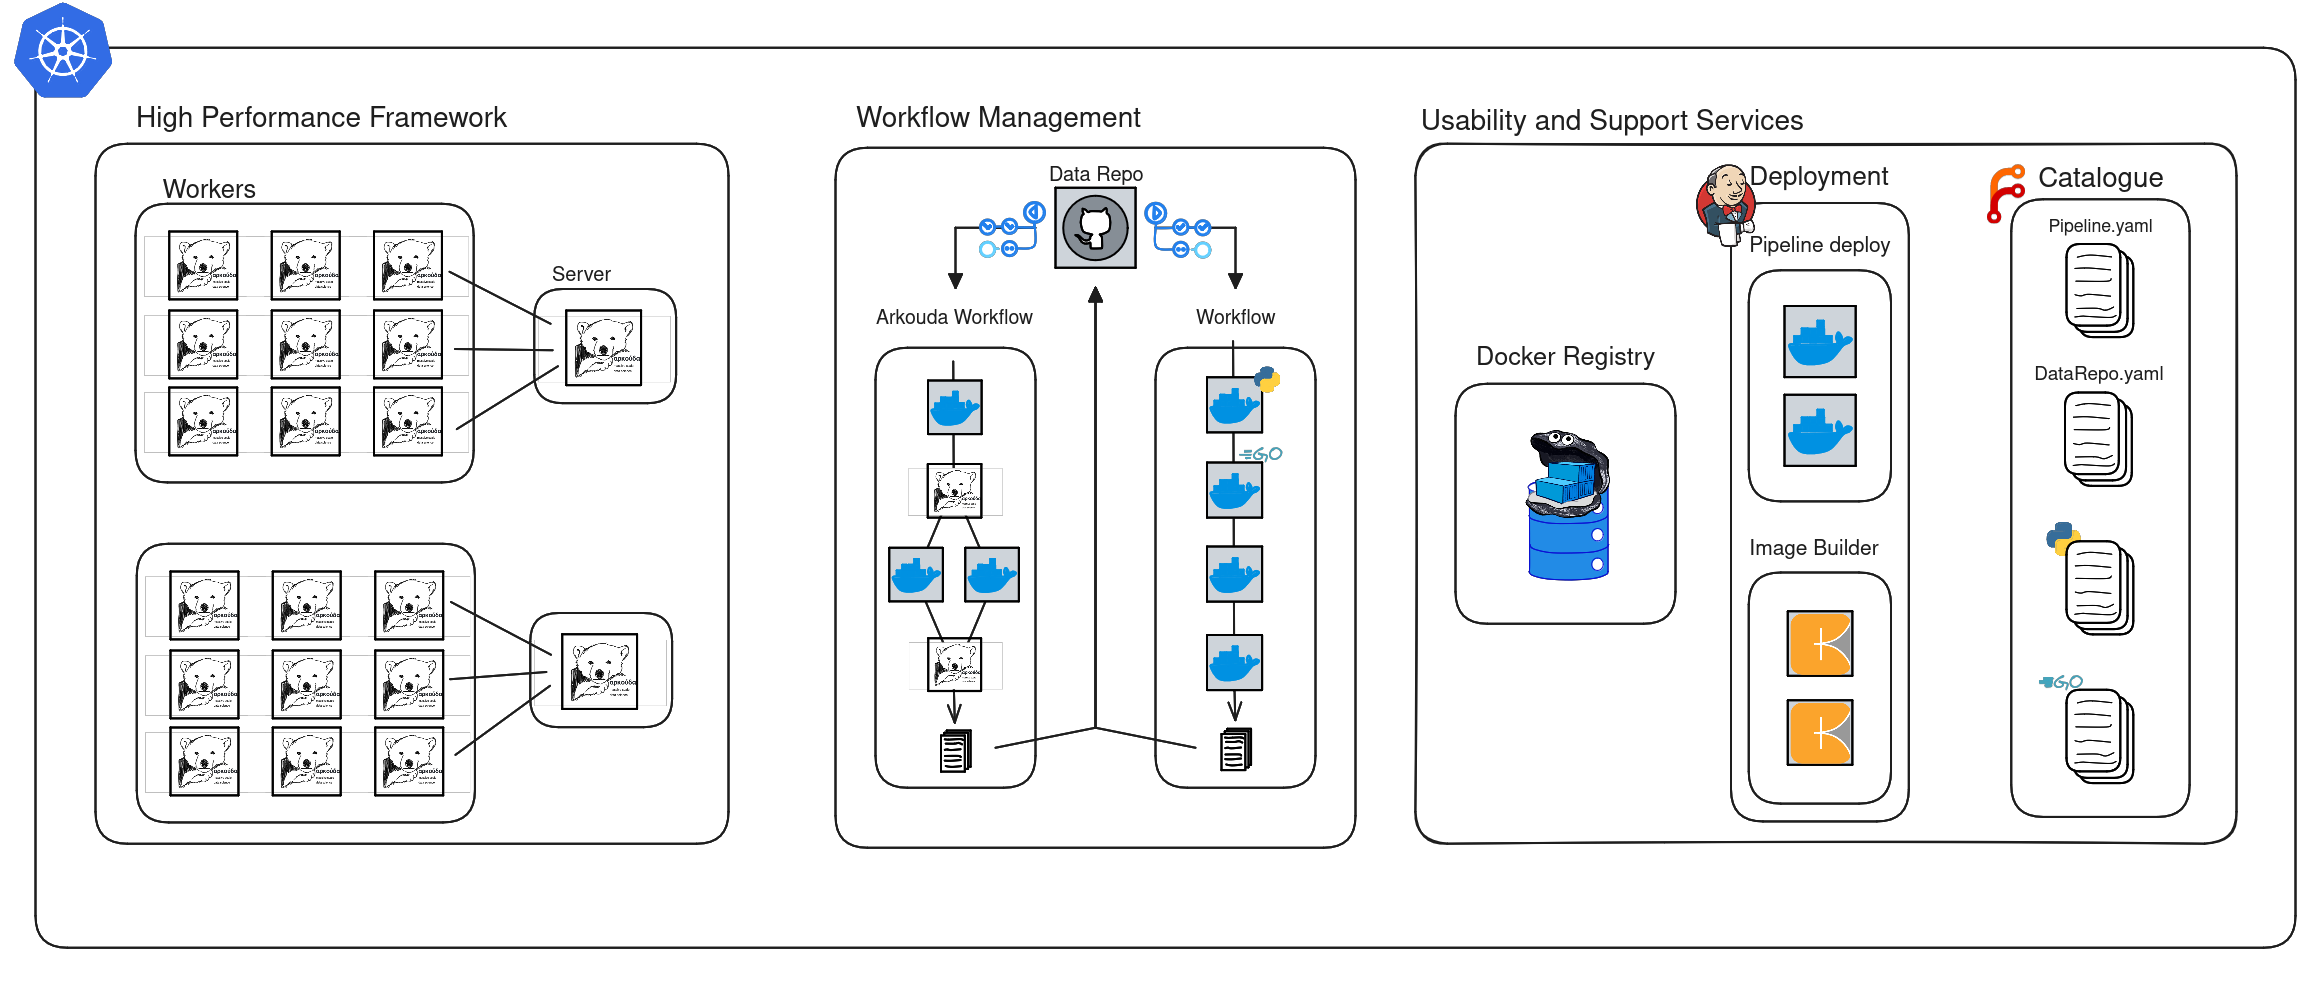
\includegraphics[width=16cm]{graphics/pachykouda_three_aspects.png}
    \caption[Pachykouda high level diagramm showing three main aspects]{Pachykouda high level infrastructure diagramm}
    \label{abb:pachykouda_three_aspects}
\end{figure}


\newpage


\section{Implementation of the Artifact}

This section will describe the iterative process of implementing the larger artifact and is broken up into 3 subsections.
While these steps where happening concurrently, they each address a different aspect of the project and therefore underwent their own iterative processes.


\subsection{Infrastructure}

\subsubsection{Minikube}

\subsubsection{Heydar Cluster}
\label{heydar_cluster}


\subsection{Usability Impovements}

\subsection{\ac{TCPP} Workloads } 


\newpage


\section{Evaluation of the Artifact}

\newpage


\chapter{Summary and Outlook}
\label{summary}
 
\section{Summary}

By way of this project paper we have assessed and described the state of the art for current technologies in the areas of 
containerized software, container orchestration and how those tie in with Software defined infrastructure.
We have done the same for the state of the art in the solution of complex problems found in the field of and  solved with \ac{HPC},
namely the two larger classes of problems, \ac{LCP} and \ac{TCP} problems, and what strategies are usually empoyed to solve those problems.

We have then addressed the problems identified by the problem statement with the statement of an initial goal, 
and structured an intervention to solve those problems by way of the creation of a prototype.
Before the iterative process of prototyping could begin we had to make a non-trivial decision on the choice of a container orchestrator/ workflow manager.
For which we defined, discussed and weighted the selection criteria, and then evaluated the available options against those criteria and 
We found our best fit through the employment of the \ac{SMART-ER} method, which was the \ac{k8s}-based orchestrator named Pachyderm.

The iterative process of prototyping was split into three main areas of focus, the infrastructure, the solution to \acp{TCP} and the integration of a complete 
\ac{CI/CD} pipeline. Each of these areas was given at least two iterations and the results of each iteration were documented, evaluated and recomendations for
future iterations were made.

The final results of the prototype were then evaluated against the initial goal and the problems identified in the problem statement,
and the resulting artifact was found to be a valid form of intervention to solve the problems identified in the problem statement,
while still being limited in scope and applicability, as was to be expected from a non production prototype. 


\section{Outlook}

% The prototype created in this project paper is a valid intervention to solve the problems identified in the problem statement,
% but still proves to have great potential for future work.
% As the time was limited and mostly spend on the furthering of the project, many avenues of high interest are still open for exploration.

% The two main areas of focus for future work are 
% the optimization of the communication stack on every level of abstraction,
% the expansion of usability functions relating to the Catalogue as these will bring the most immediate value to potential users




% ----------------------- Ende Inhalt ---------------------------------
\newpage
\chapter*{Appendix}
\addcontentsline{toc}{chapter}{Appendix}
\section*{Appendix Index}
\vspace{-8em}

% Adjust indentations before \listofanhang
\abstaendeanhangverzeichnis

\listofanhang
\clearpage
\spezialkopfzeile{Appendix} 

\lstset{
  language=TeX, % define keywords to highlight
  morekeywords={Appendix, anhangteil, anhan},
  breaklines=true,  % Enable line wrapping within the listing
  breakatwhitespace=true, % Breaks only at white space
  postbreak=\mbox{\textcolor{red}{$\hookrightarrow$}\space}, % Optional - for having a symbol at the point where text breaks
  basicstyle=\footnotesize\ttfamily, % for setting the font size/style for the code
  tabsize=2, % sets default tabsize
}


%% ================================== Discussion =======================================

\anhang{Discussion of Tool Evaluation and Weighing}

\anhangteil{Community, Support \& Docs}

This section assesses the level of external support provided for each project. To evaluate this support, we will focus on three distinct aspects and combine them into a single score. Firstly, we will examine the size of the community, as a substantial community often indicates project maturity and the availability of extensive support. As proxies for community size, we will consider two central metrics: the number of stars on GitHub and the quantity of questions on Stack Overflow.

\begin{table}[htb]
    \centering
    \caption[Community Support Data]{Community Support Data\footnotemark}
    \label{tab:community_support} 
    \begin{tabular}{|l|c|c|} 
      \textbf{Project} & \textbf{GitHub Stars} & \textbf{Stack Overflow Questions} \\ 
      Pachyderm  & 6,000   & 6          \\ 
      Argo       & 14,500  & 136        \\ 
      Clasp      & 0       & 0          \\ 
      Snaplogic  & 0       & 57         \\ 
      Airflow    & 32,200  & 10,218     \\ 
      Kubeflow   & 13,100  & 434        \\ 
      Knative    & 4,100   & 204        \\ 
      Luigi      & 16,900  & 346        \\ 
      CWL        & 1,400   & 6          \\ 
   \end{tabular}
\end{table}
\footnotetext{Data taken from GitHub and Stack Overflow on 08.11.2023}

\begin{figure}[htb]
    \centering
    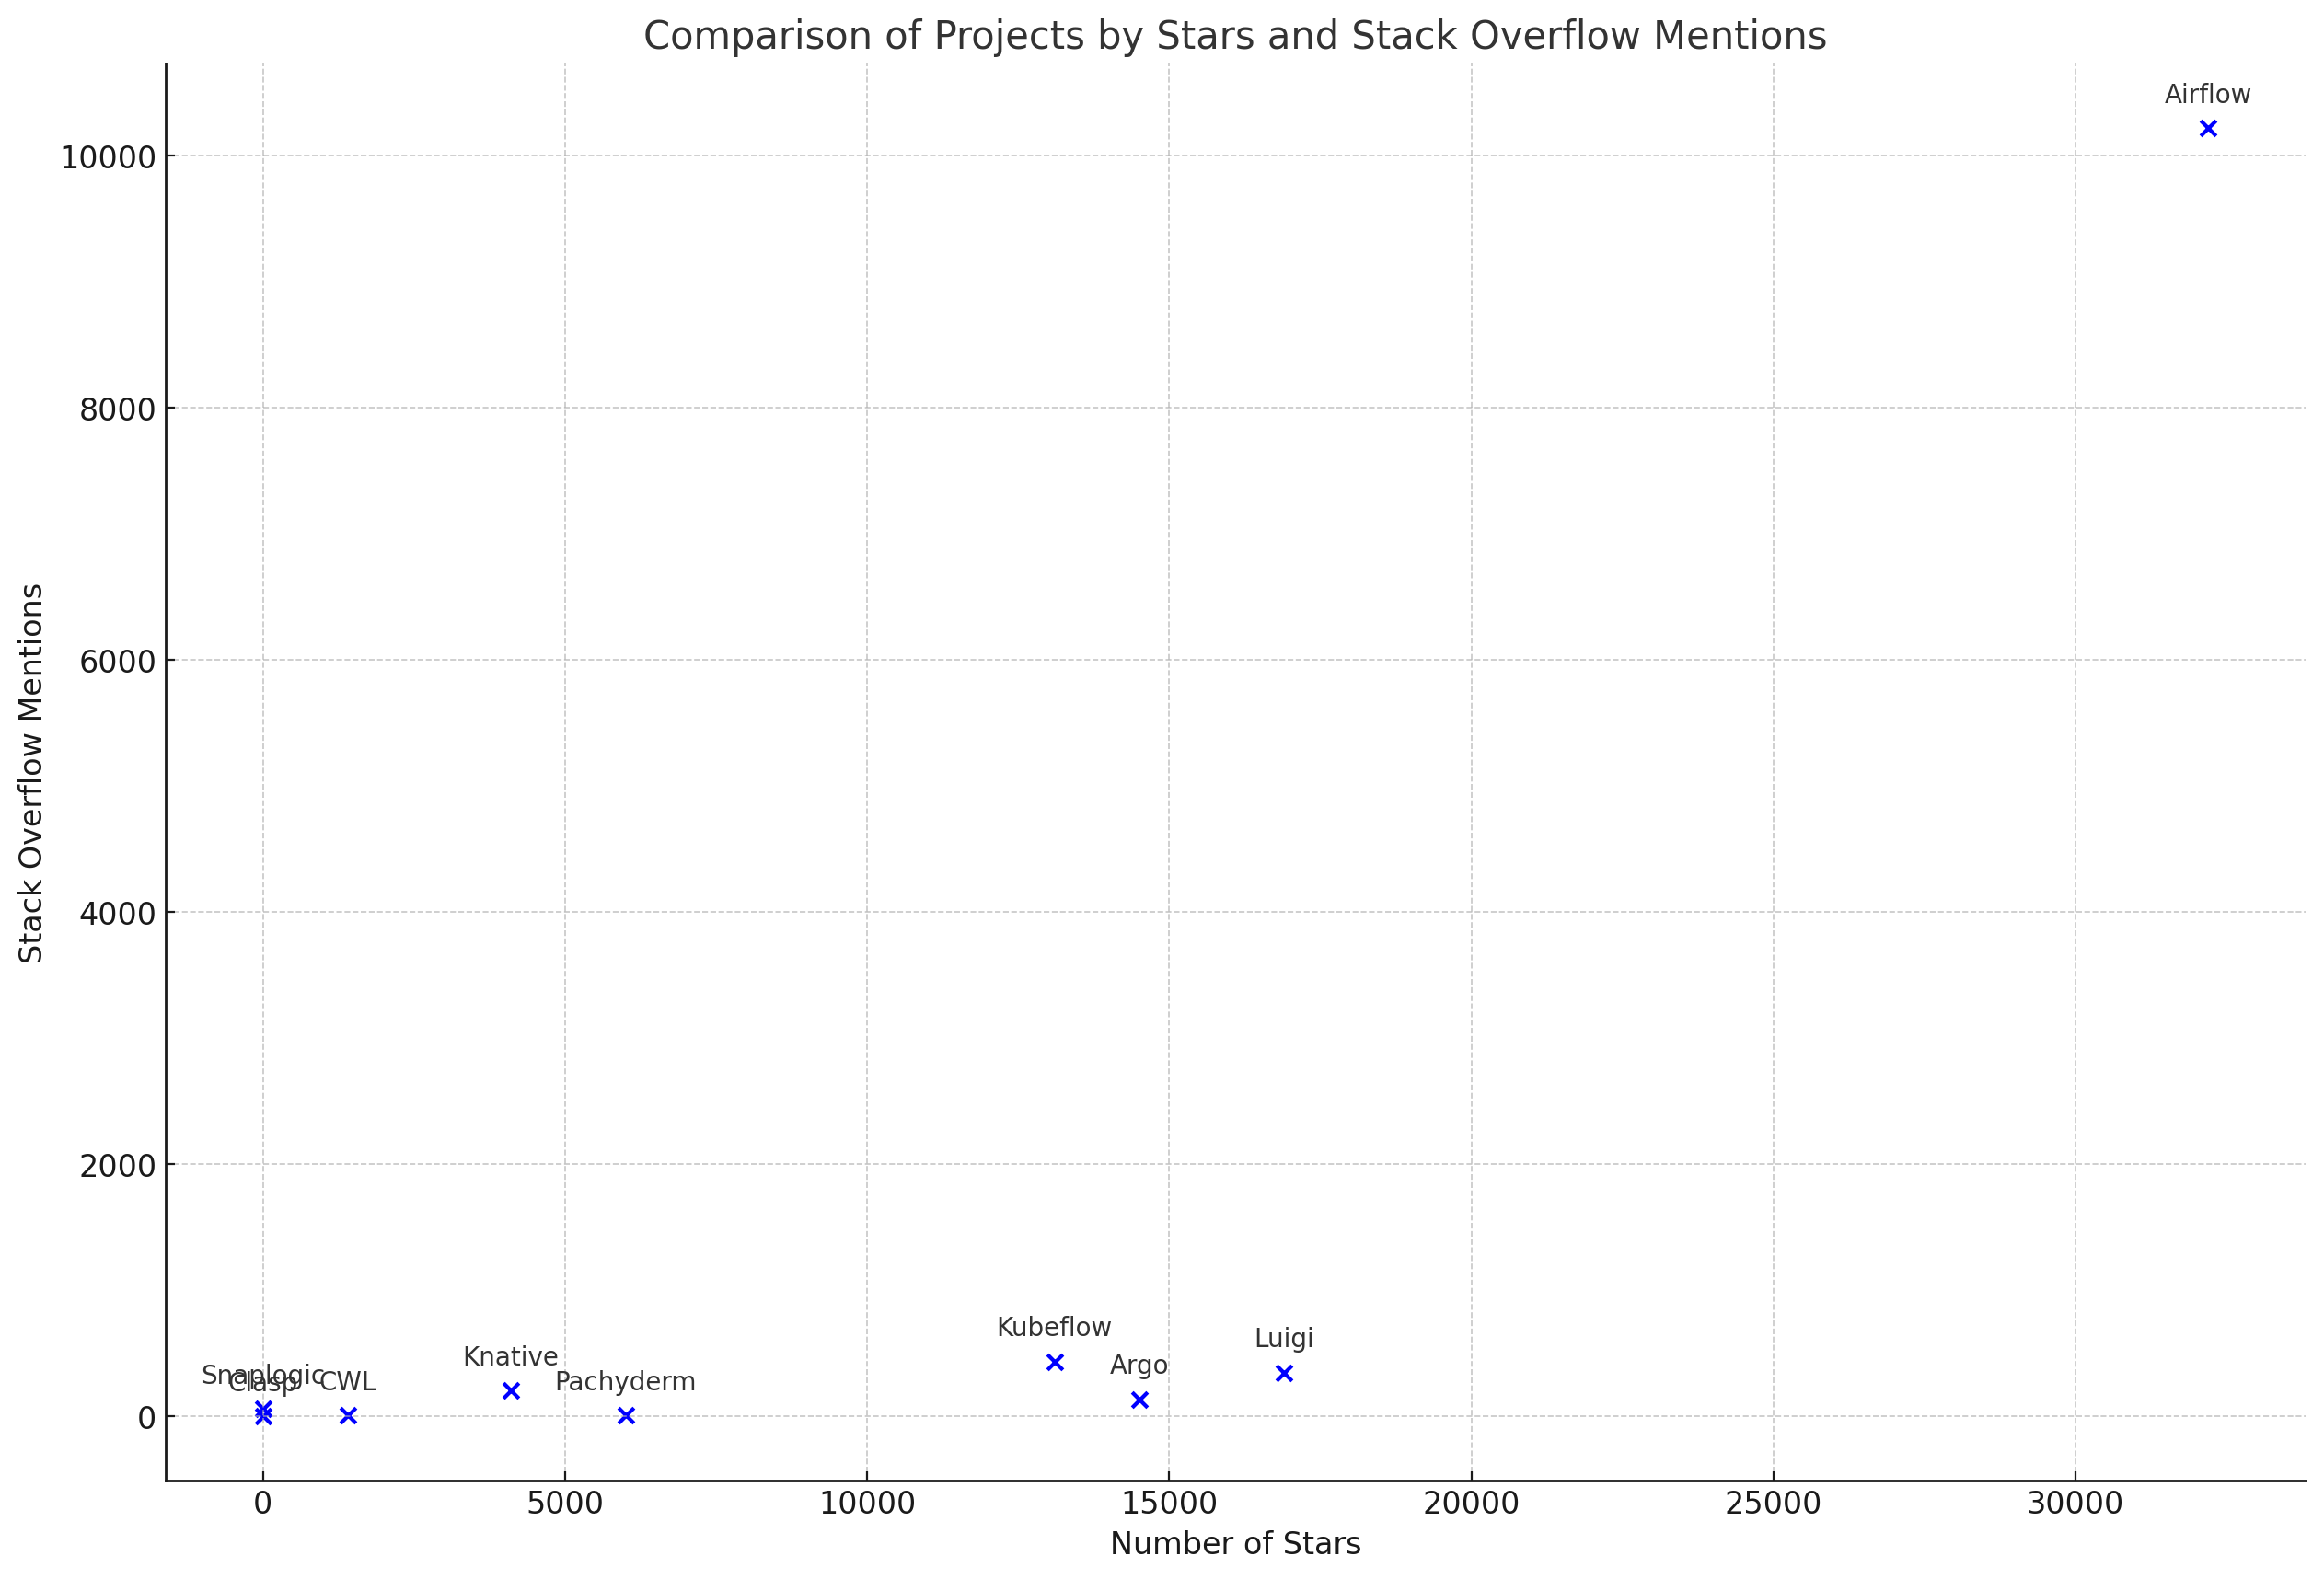
\includegraphics[width=12cm]{graphics/Stars_stackoverflow_comparison.png}
    \caption[Stars and Stack overflow Questions Comparison]{Stars and Stack Overflow Questions Comparison}
    \label{abb:stars_stackoverflow_comparison}
\end{figure}

To gauge the level of support and community engagement surrounding these projects, we have devised a composite score that normalizes and combines the GitHub stars and Stack Overflow questions metrics. The calculation of this score involves the following methodology:

Each project is represented as a point \(P_i = (x_i, y_i)\) in a two-dimensional space, with \(x_i\) and \(y_i\) being the number of GitHub stars and Stack Overflow questions, respectively, for the \(i\)-th project. The composite score \(S_i\) for each project is computed by normalizing these values to a scale of 0-10 and then taking their average.

Additionally, we acknowledge that some commercial tools, as well as certain open-source projects, offer enterprise support, reducing the reliance on the community for assistance. Similarly, projects developed in-house often have access to the original development team for support. Therefore, we will apply a flat bonus of 5 points to the scores of projects offering enterprise support and a flat bonus of 2.5 points to projects developed in-house.

\[S_i = \frac{1}{2} \left( \frac{x_i - \min(x)}{\max(x) - \min(x)} \times 10 + \frac{y_i - \min(y)}{\max(y) - \min(y)} \times 10 \right) + B_i \]

Here, \(\min(x)\), \(\max(x)\), \(\min(y)\), and \(\max(y)\) represent the minimum and maximum values of GitHub stars and Stack Overflow questions across all projects, respectively. The final scores \(S_i\), along with the respective bonuses \(B_i\), provide a comprehensive metric for comparing project popularity, community engagement, and the availability of additional support options, all on the same scale.

\begin{table}[h!]
    \centering
    \begin{tabular}{|l|c|c|c|c|} 
    \hline
        \textbf{Project} & \textbf{Composite Score} & \textbf{Enterprise Bonus} & \textbf{Inhouse Bonus}  & \textbf{Final Score}\\
        \hline
        Airflow & 10.00 & 0 & 0 & 10.00 \\
        Pachyderm & 0.93 & 5 & 2.5 & 8.43 \\
        Snaplogic & 0.03 & 5 & 0 & 5.03 \\
        Luigi & 2.79 & 0 & 0 & 2.79 \\
        Clasp & 0.00 & 0 & 2.5 & 2.5 \\
        Argo & 2.32 & 0 & 0 & 2.32 \\
        Kubeflow & 2.25 & 0 & 0 & 2.25 \\
        Knative & 0.74 & 0 & 0 & 0.74 \\
        CWL & 0.22 & 0 & 0 & 0.22 \\
    \hline
    \end{tabular}
    \caption{Composite scores of Workflow managers, sorted by final score}
    \label{tab:results}
\end{table}

\anhangteil{License}

As discussed in section \ref{crit:license} the tools in consideration should not be too restrictive.
To evaluate the criteria we will employ a 4 bucket system: 
\begin{itemize}
    \item \textbf{Ideal Situation (Score: 10):} 
    This refers to cases where either the tool is in the public domain (and therefore not subject to copyright restrictions) or where our organization possesses a direct ownership or significant influence over the licensing terms.
    This situation provides the most flexibility, allowing for extensive modification, redistribution, and proprietary use without concern for licensing infringements.


    \item \textbf{Permissive License (Score: 7.5):}
    Tools under licenses like MIT, BSD, or Apache 2.0 fall into this category.
    These licenses are highly permissive and generally allow for broad freedom, including modification, distribution, and private use, with minimal restrictions, often limited to liability and warranty.

    \item \textbf{Restrictive or Reciprocal Licenses (Score: 2.5):}
    Licenses such as the GPL or AGPL are more restrictive, requiring any changes to be open-sourced or contributions to be made back to the community.
    These “copyleft” licenses can be problematic in proprietary settings where modifications or integrations need to remain confidential.

    \item \textbf{Unacceptable Licenses (Score: 0):}
    This includes licenses that impose burdensome conditions or high costs, proprietary software where the source code is unavailable, or situations where the licensing terms make it impractical to use within our projects.
    For instance, licenses that mandate the purchase of additional software, restrict certain types of use, or pose potential legal risks would fall into this category.
\end{itemize}

Now we will evaluate the licenses of the tools in question, and assign them a score based on the above criteria.

\begin{itemize}
    \item \textbf{Pachyderm} 
    The licensing model of Pachyderm follows a model which has similarities with the "Open Core model" \footcite{PahcydermPricing2022}.
    Which means that while the core functionalities are published as the "COMMUNITY EDITION" with a permissive source-available License (Apache License 2.0) \footcite{PachydermLICENSEMaster}.
    Functionality like \ac{SSO} or the ability to create more than 16 pipelines are part of a different distribution under a Commercial License.

    But in our case this is of no concern, as the startup behind the Pachyderm software, including its \ac{IP} was acquired by \ac{HPE}.
    Giving us a free hand to modify without needing to worry.

    \item \textbf{Argo}Argo's adoption of the Apache License 2.0 \footcite{ArgocdLICENSEMaster} aligns with common practices for open-source projects, affording users considerable freedom. This permissive license simplifies the use, modification, and redistribution of the software, an aspect that's particularly beneficial for collaborative development or integration into proprietary software. Given our requirements and operational context, this offers us the flexibility needed for adaptation and potential enhancements without stringent restrictions, streamlining any developmental efforts we undertake with Argo.
    \item \textbf{\ac{CLASP}} is not a published software and therefore not under any specific license.
    But similar considerations as the ones of Pachyderm apply here as well, as it is an internal project the \ac{IP} also completely belongs to \ac{HPE}

    \item \textbf{Snaplogic} is an entirely commercial product which does not provide insight into nor the right to modify their Software \footcite{SnapLogicMasterSubscription}.
    But as they might agree this is not a total knockout criterion for this entire project, but in regard to the licensing it will be weighted with 0.
    \item \textbf{Airflow} is licensed under the Apache License 2.0. \footcite{LicenseAirflowDocumentation}
    \item \textbf{Kubeflow} is licensed under the Apache License 2.0. \footcite{KubeflowLICENSEMaster}
    \item \textbf{Knative} is licensed under the Apache License 2.0. \footcite{KnativeDocsLICENSE}
    \item \textbf{Luigi} is licensed under the Apache License 2.0. \footcite{LuigiLICENSEMaster}
    \item \textbf{CWL} is licensed under the Apache License 2.0. \footcite{CwlutilsLICENSEMain}
    
\end{itemize}

\anhangteil{Strategic alignment}

When considering the strategic alignment within the context of \ac{HPE} the goal is to ensure that the tool can be used in combination with or as extension to the Products \ac{HPE} is offering.
Tools that have been developed by the company in the first place or have been acquired by \ac{HPE} must be of a high strategic value to the company, as otherwise they would not have been developed or acquired in the first place.

This is especially true for Pachyderm, as it has been acquired in 2023 \footcite{HewlettPackardEnterprise} as part of their realignment towards hybrid cloud provider.
The eight years since the development of \ac{CLASP} in 2015 \footcite{sayersCLoudApplicationServices2015} the priorities of somewhat shifted, its concept is still relevant and was originally developed by the labs to fill a strategic gap.

While some of these tools might have been used in other projects, been contributed to by \ac{HPE} employees or are supported on the Ezmeral platform, they are not part 
of the core product portfolio and therefore not of strategic importance.

One thing that would have to be considered is the way one would make oneself dependant of the company, as \ac{HPE} would have to enter into negotiations with the company behind Snaplogic, 
this state of dependency an the need to find a compromise would be a strategic disadvantage.

Therefore the following scores have been assigned:

\begin{table}[htb]
  \centering
  \caption{Strategic Alignment Scores}
  \begin{tabular}{|l|c|} 
    \textbf{Project} & \textbf{Strategic Alignment} \\
    Pachyderm  & 10   \\
    \ac{CLASP}       & 7.5  \\
    Argocd       & 2.5  \\
    Snaplogic      & 0          \\
    Airflow      & 2.5          \\
    Kubeflow      & 2.5          \\
    Knative      & 2.5          \\
    Luigi      & 2.5          \\
    CWL      & 2.5          \\
  \end{tabular}
\end{table}

\anhangteil{Ease of Use}

\anhangteil{Maturity}

The evaluation of the tools is centrally based on their open source repositories, as this is the most accessible and transparent source of information.
In order to evaluate the maturity of the tools, we will look at the age, the number of commits, the ratio of commits to age, the number of closed issues and the ratio of closed issues to open issues.
We will then combine these metrics into a single score, which will be used to evaluate the maturity of the tools. Products like Snaplogic, which are not open source,
as they are a commercial product it is to be expected that they are somewhat mature, as they are already being used in production environments and are used by many companies.


\begin{table}[htb]
  \centering
  \label{tab:maturity_data}
  \begin{tabular}{|l|c|c|c|c|c|}
    \hline
    \textbf{Project} & \textbf{Age (Days since 08.11.2023)} & \textbf{Commits} &  \textbf{ Open Issues} & \textbf{Closed Issues} \\
    \hline
    Pachyderm  & 3352 & 22143 & 889 & 2387  \\
    Argo      & 2098 & 6047  & 2693 & 4161 \\
    Airflow    & 3131 & 22026 & 762 & 7467 \\
    Kubeflow   & 2168 & 2514  & 178 & 3615 \\
    Knative    & 2113 & 8531  & 202 & 4332 \\
    Luigi      & 4066 & 4088  & 93  & 879  \\
    CWL        & 2954 & 4512  & 421 & 358  \\
    \hline
 \end{tabular}
 \caption[Maturity Data]{Maturity Data\footnotemark}
\end{table}
\footnotetext{Data taken from GitHub on 08.11.2023}


How these values compare to each other in normalized form is shown in the following graphs:

\begin{figure}[H]
  \centering
  \begin{minipage}{.5\textwidth}
    \centering
    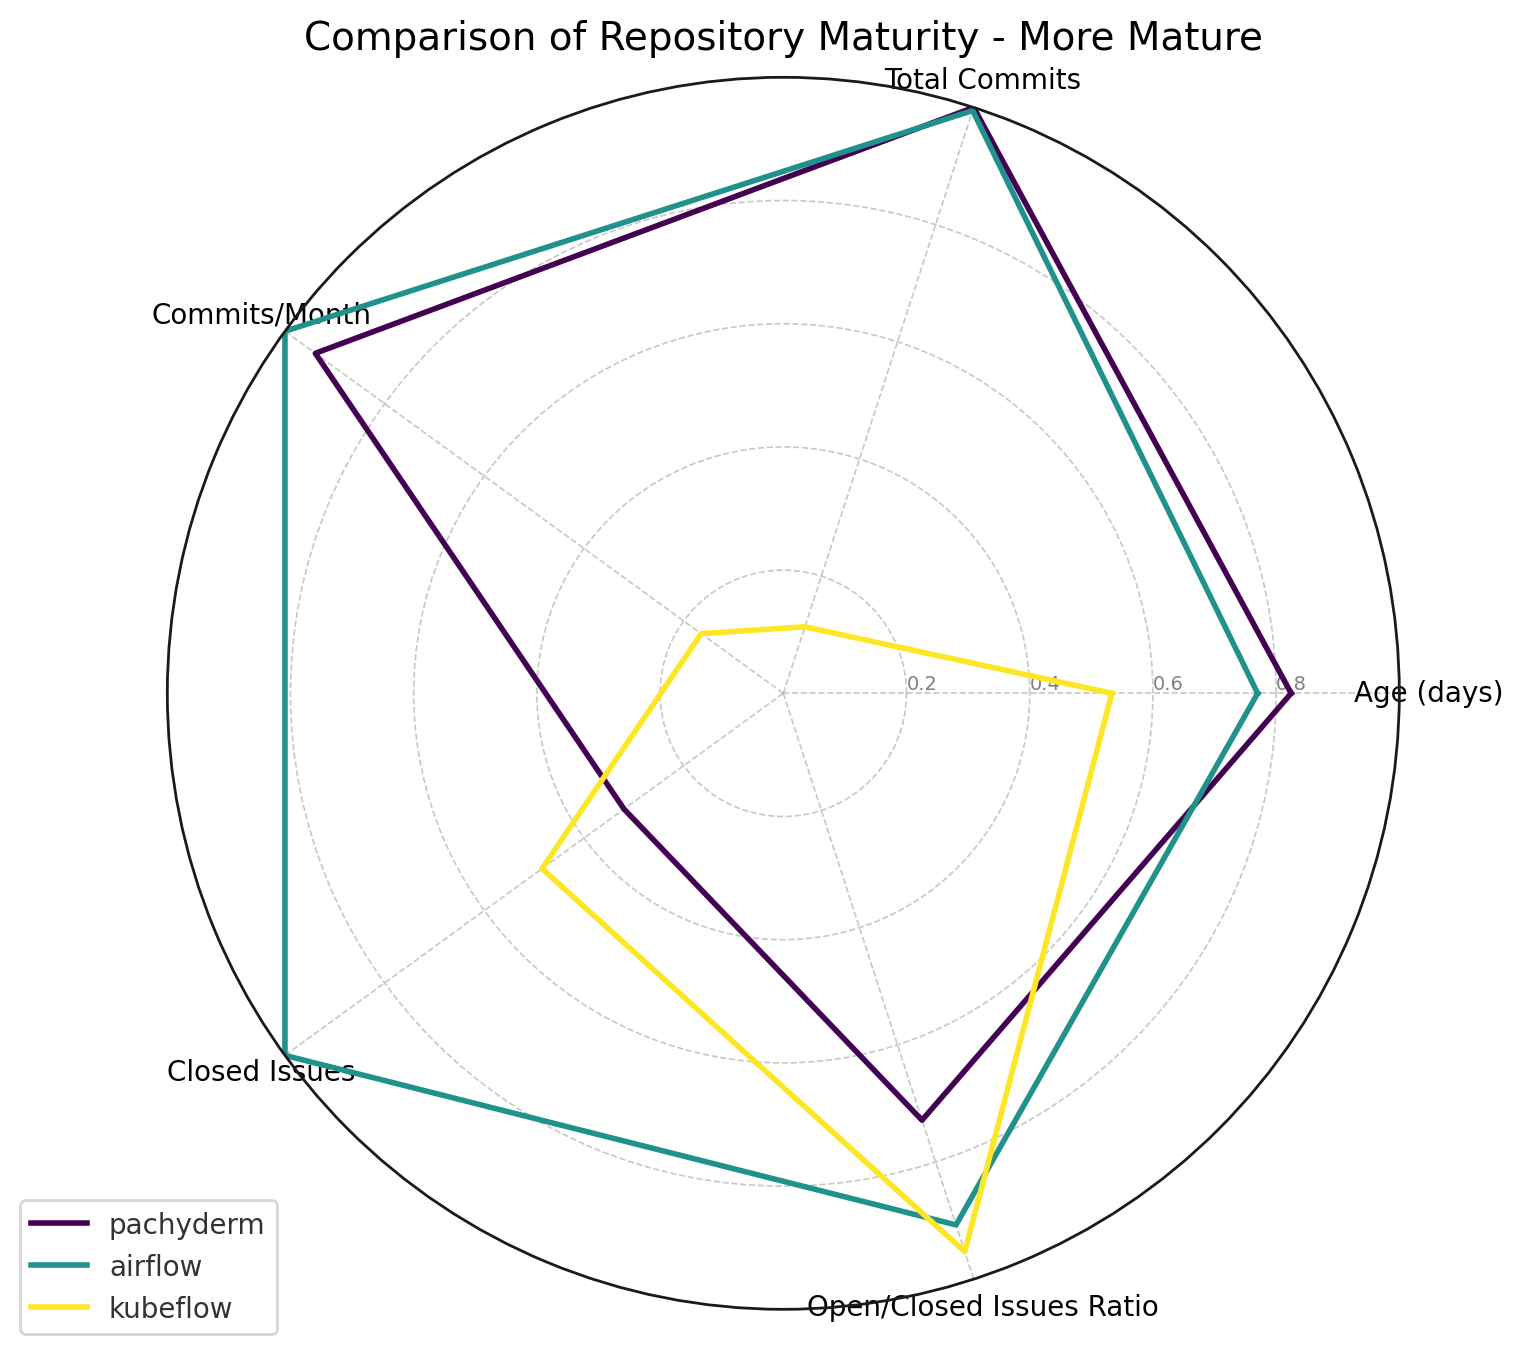
\includegraphics[width=6cm]{graphics/Maturity_graph_larger.png}
    \caption[Maturity Metric comparison (higher rated projects)]{Maturity Metric comparison}
    \label{abb: maturity_metric_comparison_larger}
  \end{minipage}%
  \begin{minipage}{.5\textwidth}
    \centering
    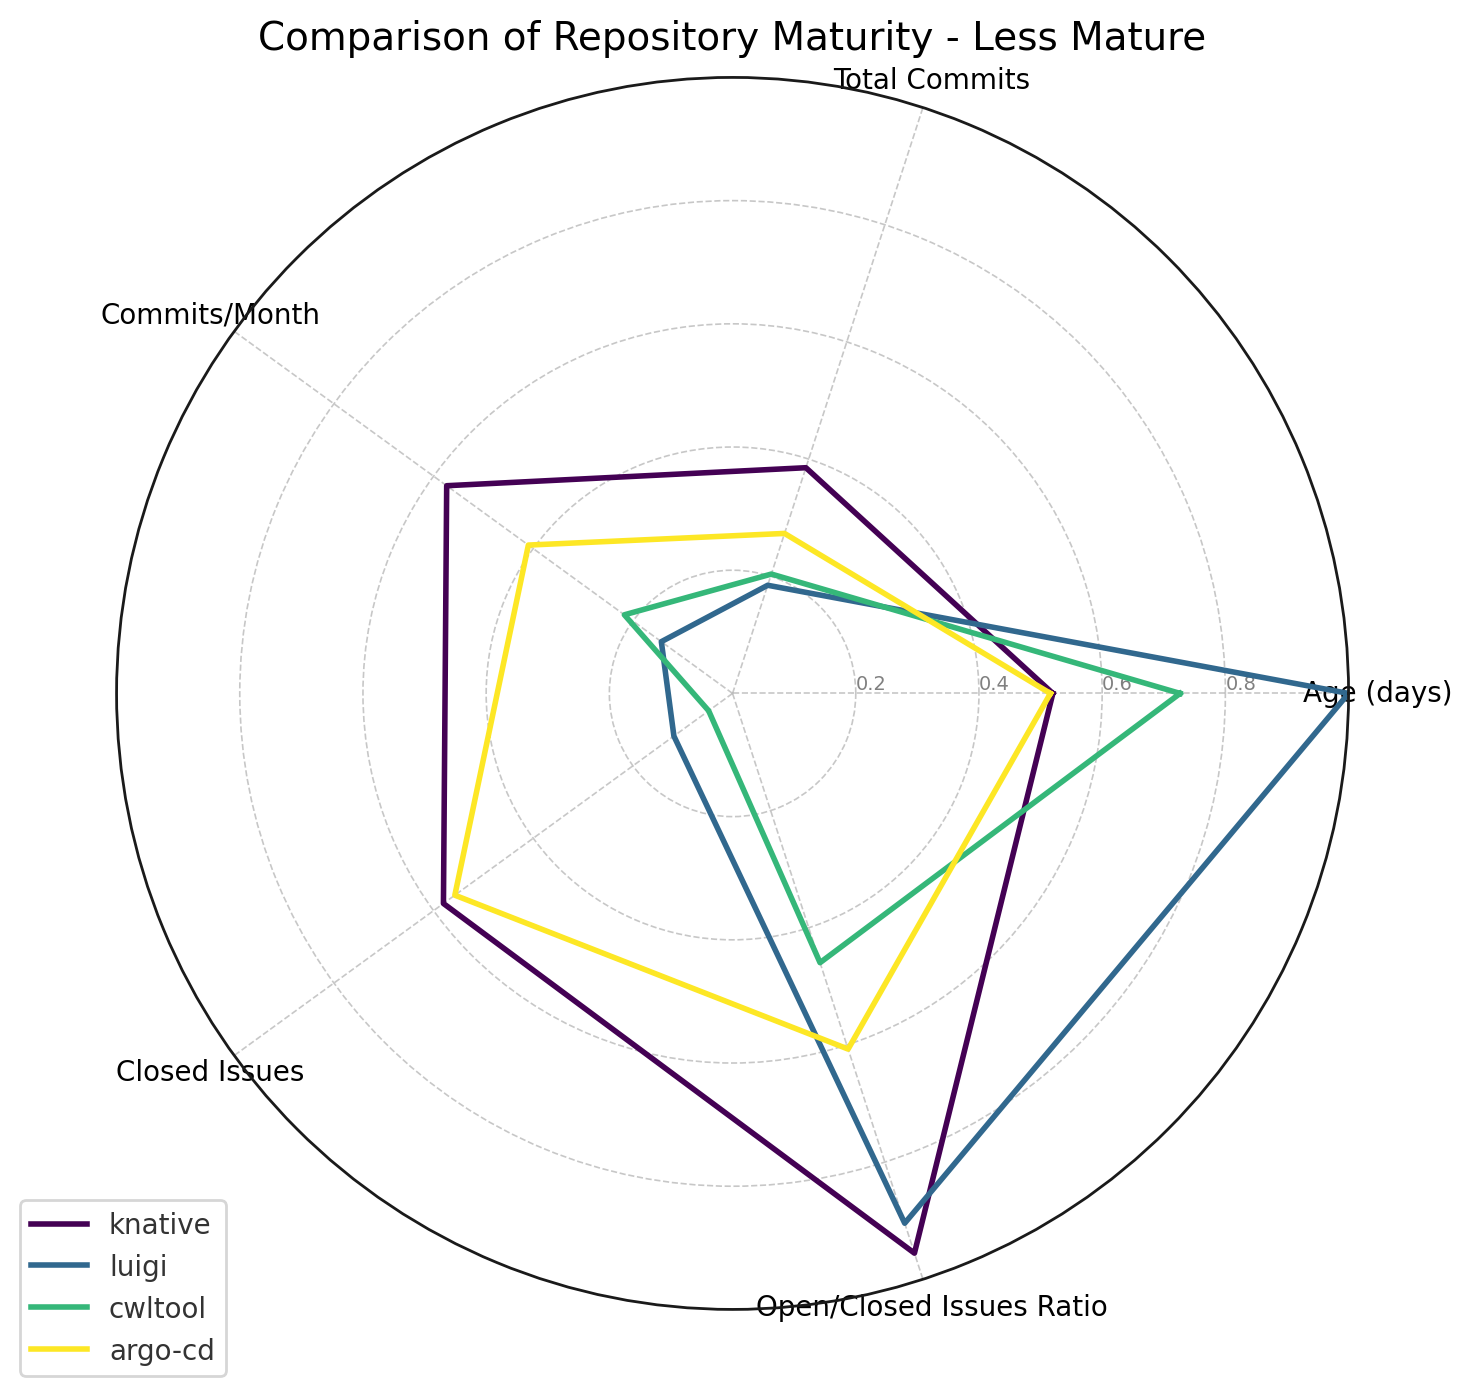
\includegraphics[width=6cm]{graphics/Maturity_graph_smaller.png}
    \caption[Maturity Metric comparison (lower rated projects)]{Maturity Metric comparison}
    \label{abb: maturity_metric_comparison_smaller}
  \end{minipage}
\end{figure}


The combined maturity score for each tool is calculated as follows:


\begin{itemize}
  \item Age (days): Current Date - Created Date
  \item Commits/Month: Total Commits / (Age in months)
  \item Open/Closed Issues Ratio: Closed Issues / (Open Issues + Closed Issues)
  \item Normalized Metrics: Each metric is normalized by dividing by the maximum value among all repositories.
  \item Combined Maturity Score: Average of normalized metrics, scaled to a 1-10 range as \( 1 + (9 \times \text{average}) \).
\end{itemize}

\begin{table}[htb]
  \centering
  \caption{Maturity Scores}
  \begin{tabular}{|l|c|} 
    \textbf{Project} & \textbf{Maturity Score} \\
    Pachyderm  & 7.86   \\
    Argo       & 5.2  \\
    Airflow    & 9.41  \\
    Kubeflow   & 5.05  \\
    Knative    & 6.43  \\
    Luigi      & 5.23  \\
    CWL        &  3.98 \\
  \end{tabular}
\end{table}

\anhangteil{Cost}

This section aims to compare the relative cost of the products in relation to each other.
We previously factored in the enterprise features, so when enterprise support is available and applicable we will take this into consideration.
Here we have three categories of products first those which are completely free and without any enterprise support,
secondly those which are free but offer enterprise support and lastly those which operate on a subscription basis.
To address various cost models, we classify the tools into the following categories:

\begin{enumerate}
  \item \textbf{Open-source and Community-Supported Tools (No Cost):} Free tools, typically open-source, relying on a community for maintenance.
  \item \textbf{Open-source with Optional Enterprise Support (Variable Cost):} Open-source with paid enterprise support offering advanced features by the developing team.
  \item \textbf{Commercial Products (Subscription-Based Cost):} Tools that require ongoing payment for use depending on the level of service and feature access.
\end{enumerate}


\begin{table}[htb]
  \centering
  \caption{Scores Based on Cost}
  \label{tab:cost_scores}
  \begin{tabular}{|l|c|}
    \hline
    \textbf{Project} & \textbf{Cost Score} \\
    \hline
    Airflow        &  10 \\
    Pachyderm      &   6  \\
    Snaplogic      &   3  \\
    Luigi          &  10 \\
    CLASP          &  10 \\ 
    Argo           &  10 \\
    Kubeflow       &  10 \\
    Knative        &  10 \\
    CWL            &  10 \\
    \hline
  \end{tabular}
\end{table}




%% ============================== Diagrams =====================================

\newpage
\anhang{Diagrams}

\anhangteil{Lookup table weighing functions}

\begin{figure}[H]
  \centering
  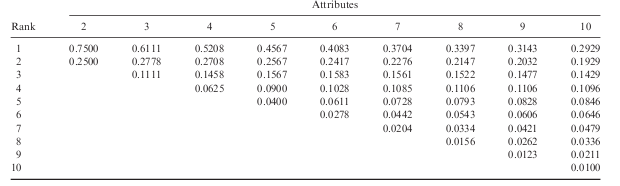
\includegraphics[width=16cm]{graphics/ROC_weights.png}
  \caption[ROC weights]{ROC weights \footnotemark}
  \label{abb:Roc_weights}
\end{figure}
\footnotetext{Taken from: \cite{robertsWeightApproximationsMultiattribute2002a}}


\begin{figure}[H]
    \centering
    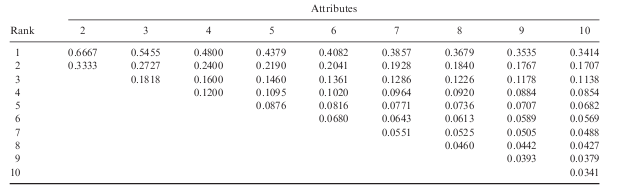
\includegraphics[width=16cm]{graphics/RR_weigths.png}
    \caption[RR weights]{RR weights \footnotemark}
    \label{abb:RR_weights}
  \end{figure}
  \footnotetext{Taken from: \cite{robertsWeightApproximationsMultiattribute2002a}}
  
\begin{figure}[H]
    \centering
    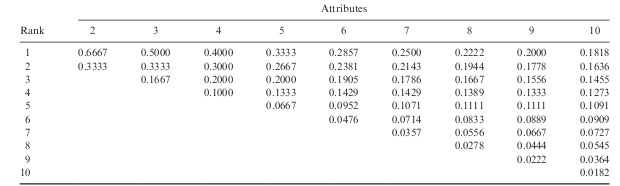
\includegraphics[width=16cm]{graphics/RS_weigts.png}
    \caption[RS weights]{RS weights \footnotemark}
    \label{abb:RS_weights}
  \end{figure}
  \footnotetext{Taken from: \cite{robertsWeightApproximationsMultiattribute2002a}}
  


\anhangteil{Pipeline Communication Swim Lane Diagram}
\begin{figure}[H]
  \centering
  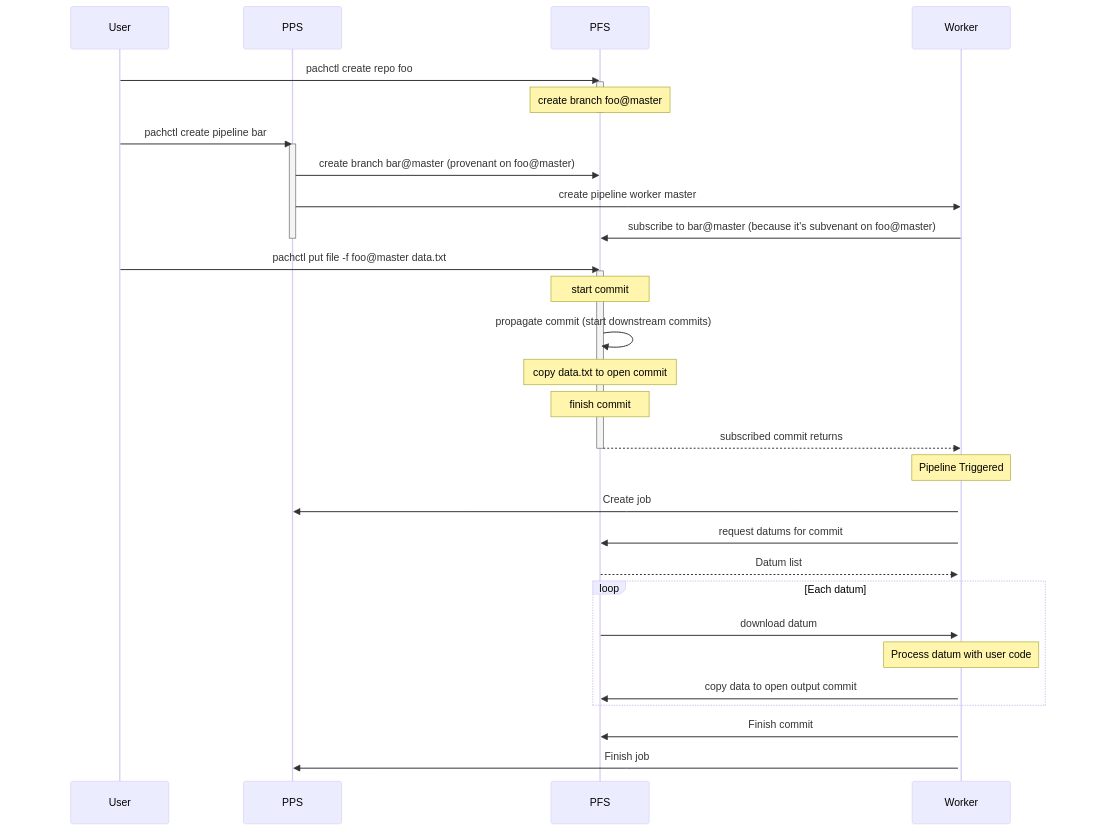
\includegraphics[width=14cm]{graphics/pipeline_communication_sld.png}
  \caption[Swim lane Diagram of the communication between the user and Pachyderm]{Swim lane Diagram of the communication between the user and Pachyderm\footnotemark}
  \label{abb:pipeline_communication_sld}
\end{figure}
\footnotetext{Taken from: \cite{IntroPipelines2023}}

\newpage


%% ================================ README and Installation instuctions =======================================

\anhang{Minikube installation instructions}
\label{appendix:minikube_installation_instructions}
\lstinputlisting{../quellen/minikube_installation_instructions.md}

\anhang{CI/CD installation instructions}
\label{appendix:cicd_installation_instructions}
\lstinputlisting{../../Project/Kubernetes_Setup/ci_cd/README.md}



%%% Aknowledgements %%%
% \clearpage
% \chapter*{Acknowledgements}
\label{Acknowledgements}

I would like to extend my sincerest gratitude to my supervisors, [Name] and [Name], 
for their invaluable support and guidance throughout the course of this research project.
Their insightful feedback and constructive criticism have been instrumental in shaping this paper.

I would also like to thank my friends and fellow students, Pascal Daniel und Max Kirschmann, 
for their contributions and insightful discussions that helped shape this research paper.

Additionally, I would like to acknowledge the contribution of GitHub Copilot, 
an AI-powered programming tool that provided assistance with the formulation of certain sections of this paper.
Its capabilities in generating relevant code snippets and suggestions were helpful in the completion of this project.

%%% Quellenverzeichnisse (keine Anpassung nötig) %%%
\clearpage
\literaturverzeichnis
%%% Ende Quellenverzeichnisse %%%


%%% Erklärung (keine Anpassungen nötig) %%%
% steht ganz am Ende des Dokuments
\cleardoublepage
\end{document}